% ; whizzy-master thermo-stat.tex

\def\ER{{\text{ER}}}

\chapter{BioMembrane (Plasma Membrane)}
%\chapter{Membranes}
\label{chap:membranes}
\label{cha:biom-plasma-membr}

% We have looked at the two major biomolecules: aldehyde and ketone
% (Sect.\ref{sec:aldehydes}). 
%At a higher level, a cell is a unit composition of a species, yet is very
% complicated.


To characterize the function of a cell, in this chapter, we will study
the boundary of a cell, the plasma membrane.  What are the major
functions of cellular membranes?

\begin{itemize}
\item Provide an environment for enzymes, ligands
\item A physical barriers (control traffic in/out)
\item Crucial role in mechanical property of cells
\end{itemize}


\begin{enumerate}
\item In prokaryotes, there is a single plasma membrane which contains
  hundreds of different types of proteins. These proteins (1) catalyze
  ATP synthesis and initiation of DNA replication, (2) membrane
  transport proteins that enable specific ions, sugars, amino acids,
  and vitamins to cross the impermeable phospholipid bilayer to enter
  the cell and other metabolic product to exit.

\item In eukaryotes, the plasma membrane is neither a site for ATP
  synthesis nor DNA replication. Yet it is studded with a multitude of
  membrane transport proteins that allow selective import/export of
  small molecules and ions.  Another types of proteins: (1) receptors
  are proteins that allow the cell to recognize chemical signals from
  neighboring to adjust its metabolism or its pattern of gene
  expression in response. Other specialized plasma membrane proteins
  allow the cell to adhere to other cells and to components in the
  surrounding fibrous extracellular matrix (e.g. binding components of
  the cytoskeleton).
\end{enumerate}

\section{New papers}

\citep{kusumi1996, kusumi2005}


\section{Memebrane as a natural barrier}
\label{sec:membrane-natural-barrier}

Cells use inorganic ions (\ce{K+}, \ce{Ca2+}, \ce{Na+}, \ce{Cl-}) for
transmitting signals across the cell membranes and along the surface
of the cell. However, ions have great difficulty passing through the
membranes by simple diffusion because the hydrophobic inner part of
the cell membranes that oppose the passage of hydrophilic
ions. Inorganic ions is quite small, however, there are always a layer
of water molecules attaching to it. This phenomena makes it difficult
for ion to diffuse.

A membrane is a phospholipid bilayer, i.e. two layers of phospholipid
(Sect.\ref{sec:phospholipids}) that build a hydrophobic [not disolving in
water], low dielectric barrier [dielectric material is poor conductor of
electricity and can serve as a capacitor] to hydrophilic and charged molecules.
So, the a biological membranes serves as {\it an electrical insulator}
(Sect.\ref{sec:plasmamembrane-as-RC}).

\section{1. Membrane compositions: cartoon models for plasma membranes}
\label{sec:models-membranes}
%\section{Models of biomembrane}
\label{sec:models-biomembrane}

Models for membranes:
\begin{itemize}

\item 1855: Carl N\"ageli realized the existence of an outer layer of
  cells ({\bf plasma membrane}) with its own special properties when
  he noted the difference in the rates of penetration of pigments in
  damaged and undamaged plant cells.

  \begin{figure}[htb]
    \centerline{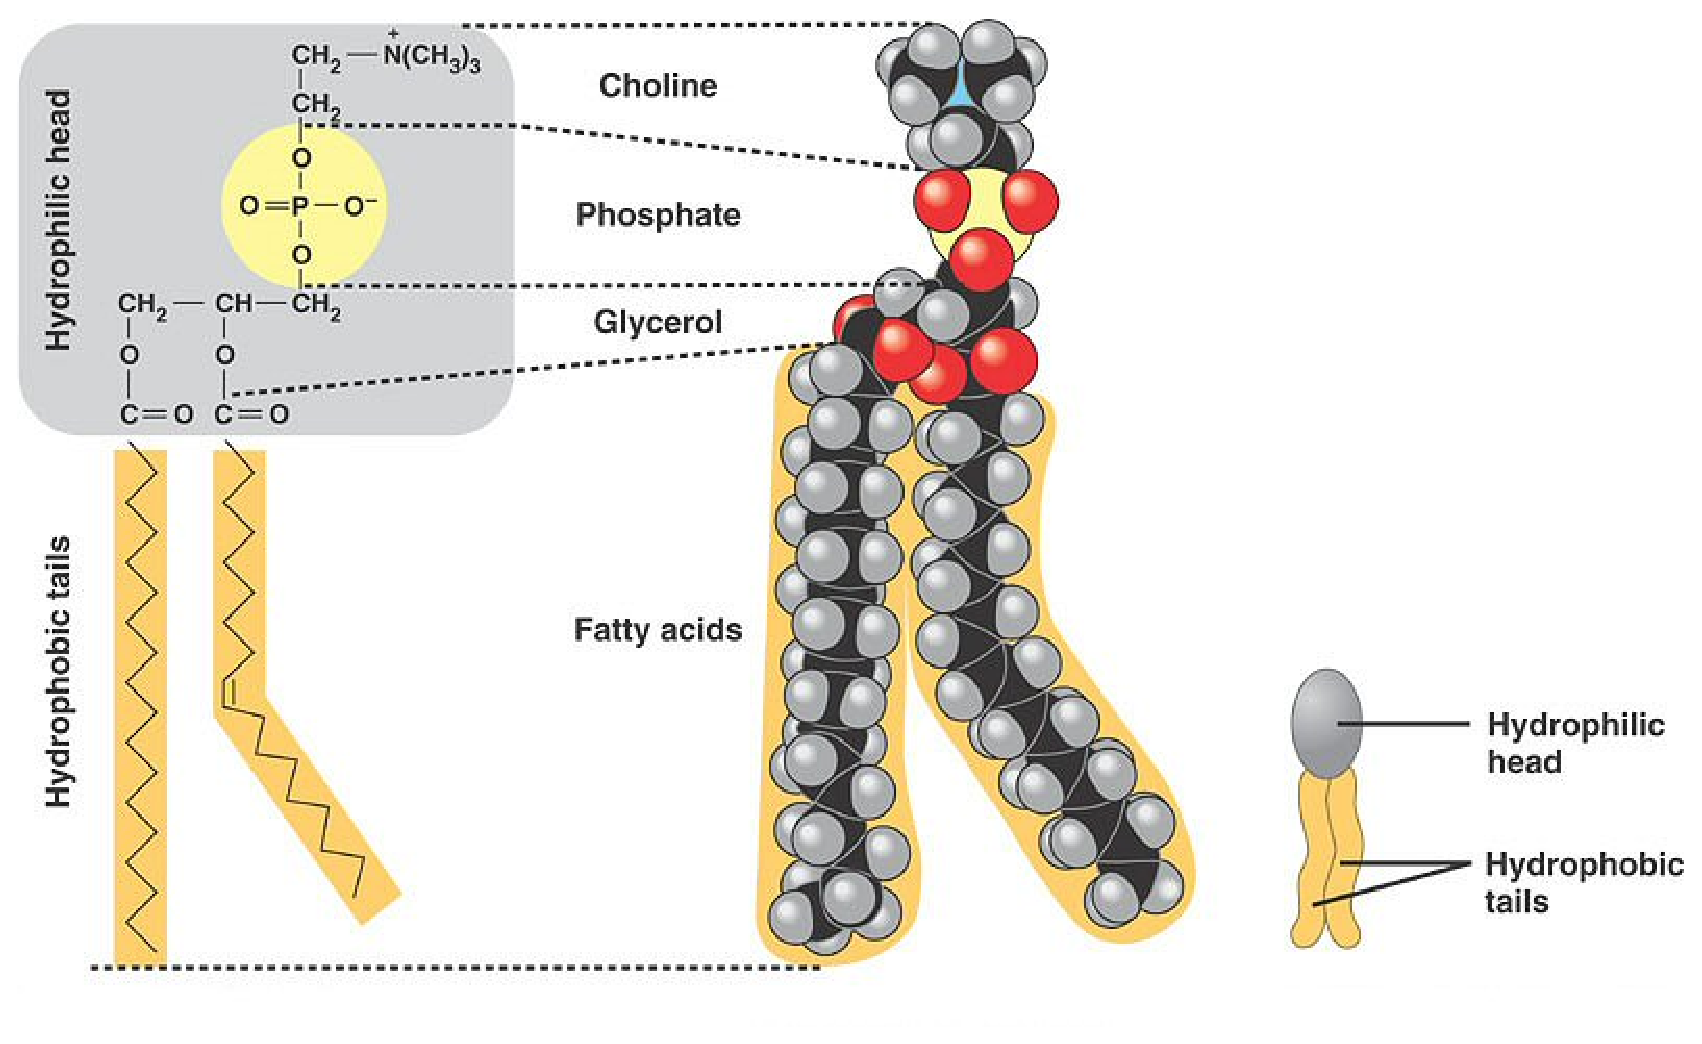
\includegraphics[height=5cm]{./images/phospholipid_structure.eps}}
    \caption{Lipids regular structure}\label{fig:lipids}
  \end{figure}

\item 1897: Wilhelm Pfeffer concluded that plasma membrane is the
  universal barrier to water and solutes. This idea was then modified
  by Charles, Overton: membranes exercise selectively control through
  its differential permeability ({\it semipermeable}) and is composed
  of certain types of liquid crystals ({\bf lipids}), as shown in
  Fig. \ref{fig:lipids}.

\item 1917: Irving Langmuir discovered that in nature, lipids tends to
  spread out into a layer of 1 molecular thick when he examined them
  close to the air-water surface.

\item 1925: Evert Gorter, Fr. Grendel noticed that the membrane of the
  erythrocyte (red blood cell) spans two lipid molecules (each
  phospholipid molecule 3nm long $\longrightarrow$ bilayer has 6nm
  thick): {\bf Gorter-Grendel lipid bilayer mode}, as shown in
  Fig.\ref{fig:membrane1}.
  \begin{figure}[htb]
    \centerline{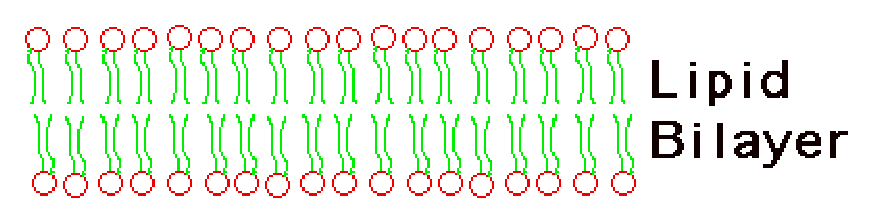
\includegraphics[height=2cm]{./images/bilayer.eps}}
    \caption{Gorter-Grendel lipids bilayer}\label{fig:membrane1}
  \end{figure}

\item mid-1930s: James Danielli, Hughe Davson, and Newton Harvey made
  accurate measurements of the {\it surface tension} of the plasma
  membrane and noticed it's lower than that of most
  lipids. Furthermore, it was known that the addition of protein to
  oil lowers the oil's surface tension. Hence, they proposed that
  {\it there are proteins on the plasma membrane}:
  {\bf Davson-Danielli
    model}\footnote{http://www.boomer.org/c/p4/c11/c1102.html}.
  Their membrane model is essentially correct. However, they believed
  that lipid bilayer located at the center and the proteins form a
  thin film at the lipid-water interfaces, as shown in
  Fig. \ref{fig:membrane2} which, later we will know that, is
  incorrect.
  \begin{figure}[htb]
    \centerline{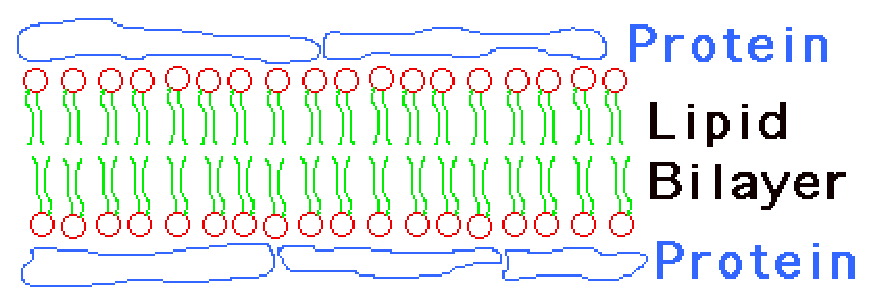
\includegraphics[height=2.5cm]{./images/bilayer-protein.eps}}
    \caption{Davson-Danielli model}\label{fig:membrane2}
  \end{figure}

\item 1954: Davson and Denielli revised the model. They proposed that
  the hydrophobic parts of the lipids lie in the bilayer interior,
  while the hydrophilic regions face the water at either side having
  proteins as gaps, as shown in \ref{fig:membrane3}.
  \begin{figure}[htb]
    \centerline{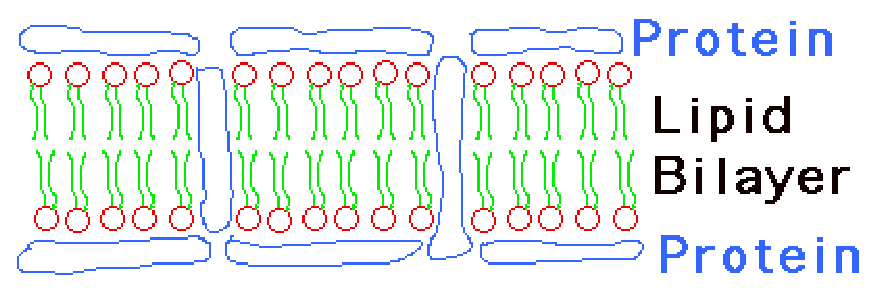
\includegraphics[height=2.5cm]{./images/bilayer-protein-modified.eps}}
    \caption{Modified Davson-Danielli model}\label{fig:membrane3}
  \end{figure}

  They also proposed the existence of small pores through the membrane
  (i.e. {\bf ion channels})
\item Mid-1950s: The bi-layer hypothesis was confirmed by the
  experiments of R.D. Robertson. He stained the membranes so that the
  two layers can be seen under electron microscope.

  \begin{figure}[htb]
    \centerline{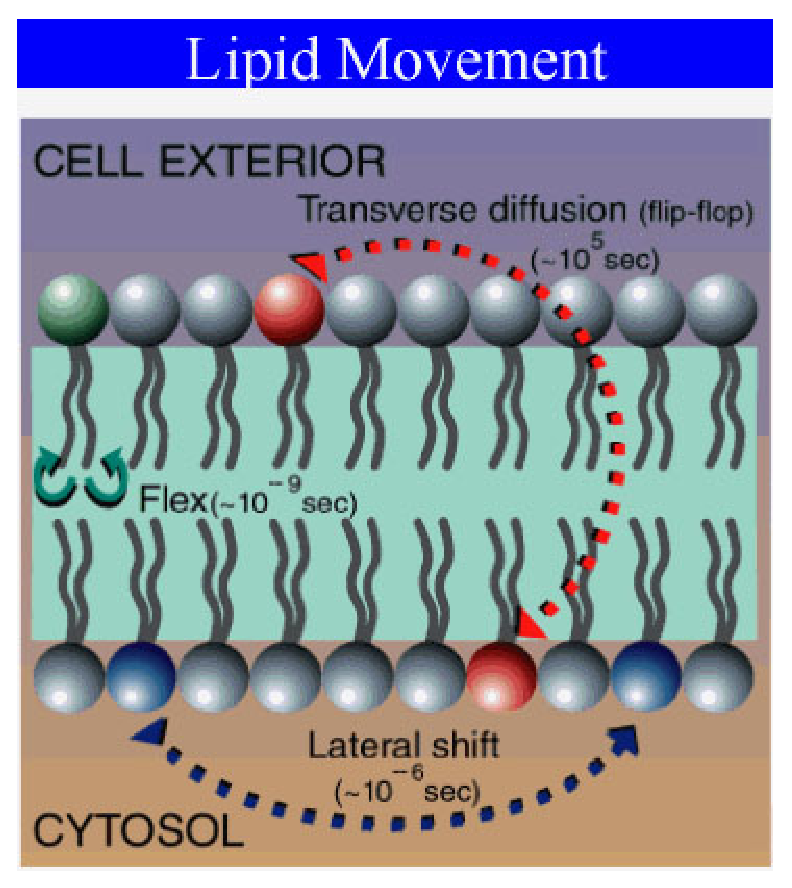
\includegraphics[height=4cm]{./images/lipidmove.eps}}
    \caption{Possible moves of lipid in the plasma membrane: lateral
      shift and (rarely) transverse diffusion }\label{fig:lipidmove}
  \end{figure}

\item 1970: David Frye and Michael Edidin detected the lateral
  movement of lipid molecules, as shown in
  Fig.~\ref{fig:lipidmove}. Molecules rarely flip transversely across
  the membrane (flip-flop process), because hydrophilic parts would
  have to cross the membrane's hydrophobic core. Phospholipids move
  quickly along the membrane's plane, about $2\mu m/s$.

\item 1970s-1980s: Singer and Nicolson suggested the
  {\bf fluid mosaic model} (Sect.\ref{sec:Singer-Nicolson}). It means that lipid
  bilayer is not rigid, yet like a fluid in which the proteins are found embedded
  in the bilayer and have freedom to move to create a {\it mosaic}
  pattern. Thus, proteins  distribute at various locations, with
  different  amounts. Proteins can drift  
  laterally, yet more slowly than
  lipids\footnote{\url{http://home.earthlink.net/~dayvdanls/CampOLs/MemModels.html}}. In
  this model, the proteins drifts between the lipids rather than
  forming a layer on either side of the lipids, as shown in
  Fig. \ref{fig:membrane4}
  \footnote{http://porpax.bio.miami.edu/~cmallery/150/memb/c8.7x7.fluid.mosaic.jpg}.
  \begin{figure}[htb]
    \centerline{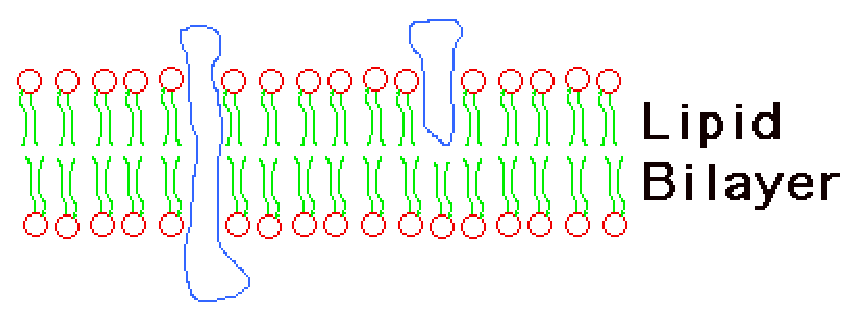
\includegraphics[height=2.5cm]{./images/fluid-mosaic-model.eps}}
    \caption{Fluid mosaic model}\label{fig:membrane4}
  \end{figure}
  The lipid-bilayers serve as both the solvent for proteins, and as a
  permeability regulator.

\item The fluic-mosaic model underwent various modifications. It's
  noted that many membranes are quite assymmetric in their lipid
  compositions. A complete illustration of the
  fluid-mosaic model is given in Fig. \ref{fig:fluid-mosaic-complete}.
  \begin{figure}[htb]
    \centerline{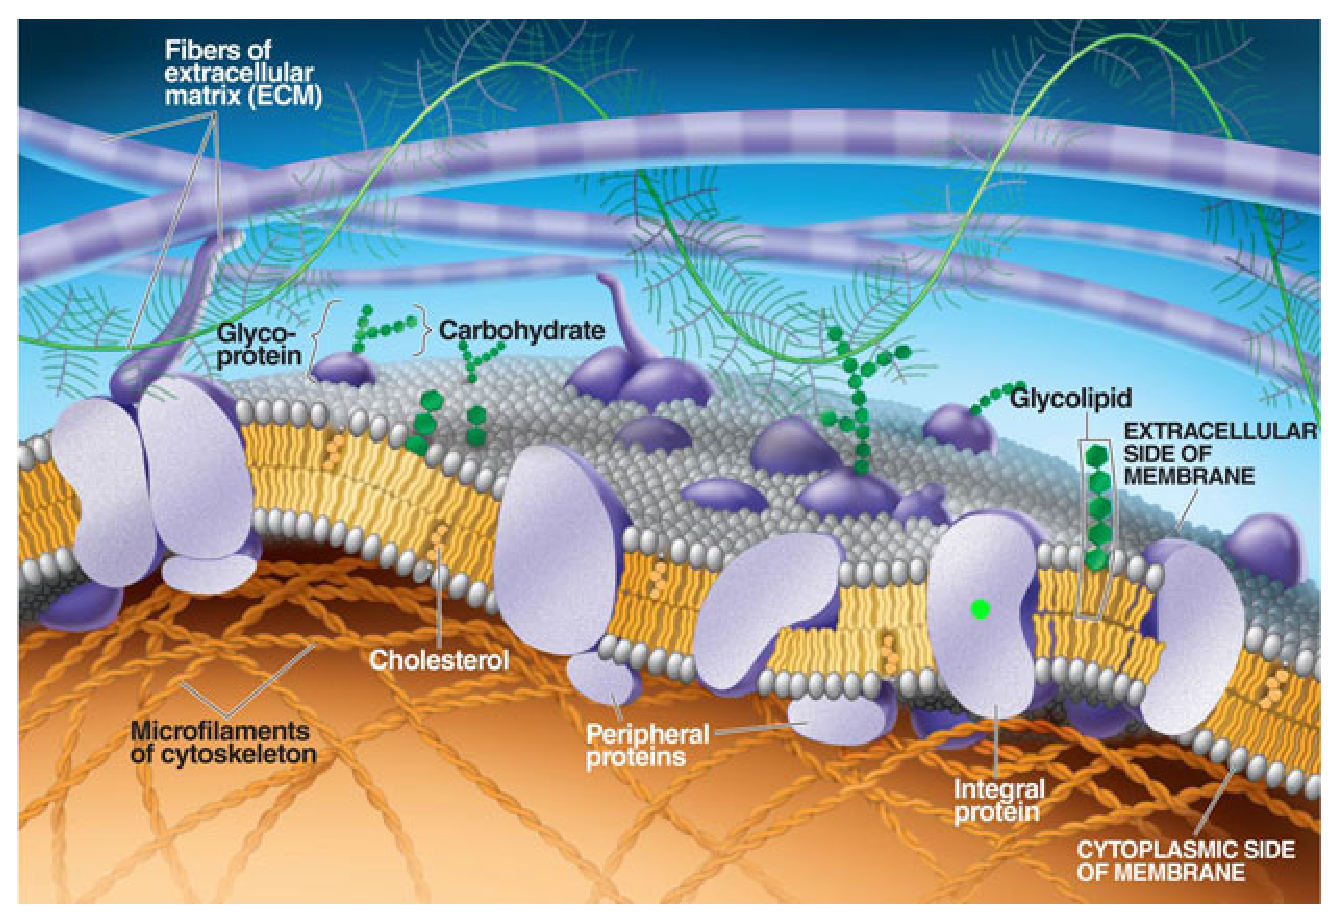
\includegraphics[height=7cm]{./images/fluid-mosaic-complete.eps}}
    \caption{Bilayer regular structure (Fluid-mosaic
      model)}\label{fig:fluid-mosaic-complete}
  \end{figure}

\item The Ole Mouritsen's {\bf matress model}
  \footnote{Mattress model of lipid-protein interactions in membranes
    Biophysical Journal, Volume 46, Issue 2, Pages 141-153
    O.MOURITSEN}
  postulated that the integral proteins often have a shorter thickness 
  than that of the bilayer. This causes local decrease in membrane
  thickness. We will know later that this is due to
  electrostatistically effect.  

\item There is a recent interest in a vesicle unit with
  membrane-bound, called {\bf liposomes} (two types: unilamellar
  liposomes \& multilamellar lipososomes). In multilamellar type, this
  structures comprises of many bilayers, arranged like the layers of
  an onion, as shown in Fig. \ref{fig:liposome}. Liposomes have a
  diameter around 30nm, and bound by a single lipid bilayer. Liposomes
  have become the standard test vehicle for experiments without
  needing the normal cellular environment. In 1974, Weissmann and his
  team developed a novel use of liposomes, i.e. for packaging enzymes
  and delivering them to deficient
  cells\footnote{http://en.wikipedia.org/wiki/Liposome}.
  \begin{figure}[htb]
    \centerline{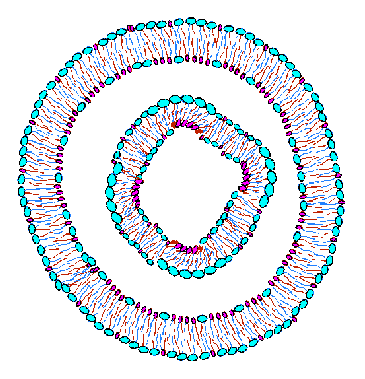
\includegraphics[height=5cm]{./images/liposome-multibilayer.eps}}
    \caption{Liposomes with two bilayers}\label{fig:liposome}
  \end{figure}
\end{itemize}

In summary, the predominant molecules in the biomembrane is {\it phospholipids}
(Sect.\ref{sec:phospholipids}). A phospholipid molecule is amphipathic, with one
head hydrophilic, and two tails hydrophobic. Other membrane lipids involve {\it
glycolipid}, which is based on {\it sphingosine molecule} - basic, long-chain,
unsaturated amino alcohol \ce{C18H37NO2} and {\it cholesterol}. Besides lipids,
the membranes also contain different types of proteins, e.g. peripheral protein,
integral protein... that serve as the sensors for cell signaling.

\subsection{Singer-Nicolson model (1972): fluid-mosaic model}
\label{sec:Singer-Nicolson}

The most widely used for the plasma membrane is {\bf fluid mosaic model}
which is proposed by Singer and Nicolson in 1972 (Singer-Nicolson
model), Fig.~\ref{fig:mosaic_fluid}.  They suggested that the
membranes are dynamic structures composed of proteins and
phospholipids. 

In this model, the phospholipid bilayer is a fluid matrix, in essence, the
solvent for protein. The proteins can be associated with the surface of this
bilayer or embedded in the bilayer to varying degrees. This corresponds to two
classes of proteins: peripheral proteins (or extrinsic proteins -
Sect.\ref{sec:peripheral-proteins}) and integral proteins (or intrinsic
proteins - Sect.\ref{sec:integral-proteins}).

\begin{itemize}
\item Peripheral proteins do not penetrate the membrane, but still
  stick to the membrane by ionic interactions or hydrogen bonds with
  integral proteins. Hence, they can be disassociated from the
  membrane by treatment with salt solutions or by changes in pH.

\item Integral proteins possess hydrophobic surface, and hence, can
  penetrate the lipid bilayer itself, as well as the surface which
  prefer the contact with aqueous medium. This type of proteins can
  either insert into the membrane or expose them on the surface of
  both sides.

\end{itemize}

\subsection{-- protein insertation rate to the membrane}

\textcolor{red}{The question is how fast can proteins move in
  biological membranes?} Many membrane proteins can move laterally
  across a membrane at a rate of a few microns per minute. On the
  other hand, some integral proteins (which often found to be anchored
  to the cytoskeleton) move very slowly, with diffusion rates of about
  10nm/sec or even slower.

The Singer-Nicolson model suggested a value of approximately 5 nm for
membrane thickness which is the same as the experimental result using
low angle X-ray difraction in a study in the early 1970s. 

The interior of these membranes are low in electron density since the
``tails" of the phospholipids are low in electron density while the
outside edges of these same membranes are of high electron density (~
high negative charged).

In the membrane, the hydrocarbon chain orientation is as follows: the
hydrocarbon tails of the phospholipids may tilt and bend and adopt
variety of orientation. However, the portions of a lipid chain near
the membrane surface lie most nearly perpendicular to the membrane
plane, i.e. the lipid chain ordering decreases toward the end of the
chain.

\subsection{The importance of assymmetry}
\label{sec:import-assymm}


Membranes are asymmetric structures (both laterally and transversely). It means
that they are not uniformly distributed.

(1) Lateral asymmetry arises when lipids or proteins of particular types cluster
in the plane of membrane.
* Lipids also undergo rapid lateral motion in membranes. Lipids in model systems
are often found in asymmetric clusters. Such behavior is referred to as a phase
separation. Lateral phase separation can be induced in model membranes by
divalent cations, which interact with negatively charged particles on the
surface of the bilayer. As shown in Figure 4, Ca2+ causes the phase separation
in these 1pids: phosphatidylserine (PS) and phosphatidylethanolamine (PE). Ca2+
added the membrane forms complexes with negatively charged serine carboxyls,
causing the PS to cluster and separate from other lipids. We call this
metal-induced lipid phase separations which have been shown to regulate the
activity of membrane-bound enzymes. It's worthy to know that there are still
other ways to alter the assymetry of lipids in biological membranes.

Figure 4. Phase separation of phosphatidylserine (green circles) induced by
divalent cations Ca2+

* One of the corollaries of the Singer-Nicolson model is that the membrane
proteins are randomly distributed through the plane of the membrane and has been
experimentally verified. However, there are cases where membrane proteins are
distributed in a nonrandom way across the surface of a membrane. Some proteins
interact intimately with certain other proteins, forming multi-subunit complexes
that perform specific functions in the membrane. A few integral membrane
proteins are known to self-associate, forming large multimeric clusters.
(2) Membrane asymmetries in the transverse direction (from one side of the
membrane to the other) can be anticipated since the properties of the membrane
depend upon which side it is. One of them is that the membrane transport, which
is driven in one direction only. One would surmise that the proteins involved in
these must be arranged asymmetrically in the membrane.
* Integral membrane proteins have been shown to arrange asymmetrically by Mark
Bretscher.
* Phospholipids are also distributed asymmetrically between the inner and outer
layer of the membranes. In erythrocyte , phosphatidylcholine (PC) comprises
about 30\% of the total phospholipid in the membrane. Of this amount, 76\% is
found in the inner monolayer, and 24\% is found in the outer monolayer, as shown
in Figure 5.

Figure 5. Distribution of different types of phospholipids across membranes
(Rothman \& Lenard, 1977, Science 194:1744) Asymmetric lipid distributions are
important to cells in several ways  -  The carbohydrate groups of glycolipids
(and of glycoproteins) always face the outside surface of plasma membrane   to
participate in cell recognition  -  The total charges on the inner and outer
surface depend on the distribution of lipids * the resulting charge difference
affects the membrane potential, which in turn is known to modulate the activity
of certain ion channels and other membrane proteins.
In summary: from a thermodynamic perspective, these asymmetries could only occur
by virtue of asymmetric syntheses of the bilayer itself or by energy-dependent
asymmetric transport mechanism. Without at least one of these, the lipids of all
kinds would eventually distribute equally.
Phospholipid can flip from oneside of the bilayer to the other by the aid of
flippase protein. With flippase, these lipids can reduce the time for it to move
from 10 days or more to a few minute or less. Rapid phospholipid movement from
one monolayer to the other occurs in an ATP-dependent manner in erythrocytes.
This energy-dependent lipid flippase activity may be responsible for the
creation and maintenance of transverse lipid asymmetries.

Figure 6. Phospholipids can be flipped across a bilayer membrane by the action
of flippase protein

We have studied phase separation which indicates lateral asymmetry. Now, we
learn phase transition which refers to the changes in a bilayer membrane under
temperature changes. The temperature at which these changes occur is called
transition temperature (~melting temperatures) Tm. Below the phase transition,
the surface area per lipid is minimal and the bilayer thickness is maximal.
Above the phase transition temperature, the surface area per lipid increases and
the bilayer thickness decrease by 10 to 15%.

Figure 7. Gel-to-liquid crystalline phase transition.

Phase transitions have been characterized in a number of pure and mixed lipid
systems.
Table 1.




\section{Lipids}
\label{sec:lipids}
\label{sec:fats}
\label{sec:fatty-acids}

Fat content in the food
\begin{verbatim}
Total fat            19g
 Saturated fat        5g
 Trans fat            5g
 Unsaturated fat      5g
\end{verbatim}

{\bf Fatty acids} are long, straight chain carboxylic acids, i.e. composed of
carbon atoms, each forming double bond to an oxygen with a string of carbons and
hydrogens attached. 
\begin{itemize}
  \item a fatty acid is saturated when all the bonds between carbon atom is
  single-bond.
\end{itemize}

A {\bf fat} (or oil) is formed when three fatty acid molecules react with a
glycerol molecule to yield a triglyceride (and three water molecules)
- Sect.\ref{sec:triglycerides}

{\bf Lipids} include a wide range of non-water soluble compounds. Fats and oils
belong to a subgroup of lipids, called glycerides, oor triglycerides to be
precise, with predominantly unsaturated fatty acids. Lipids are the essential
components in a cell membrane (Sect.\ref{sec:cell-membrane})

%We'll study its structure and classification.
\begin{figure}[hbt]
  \centerline{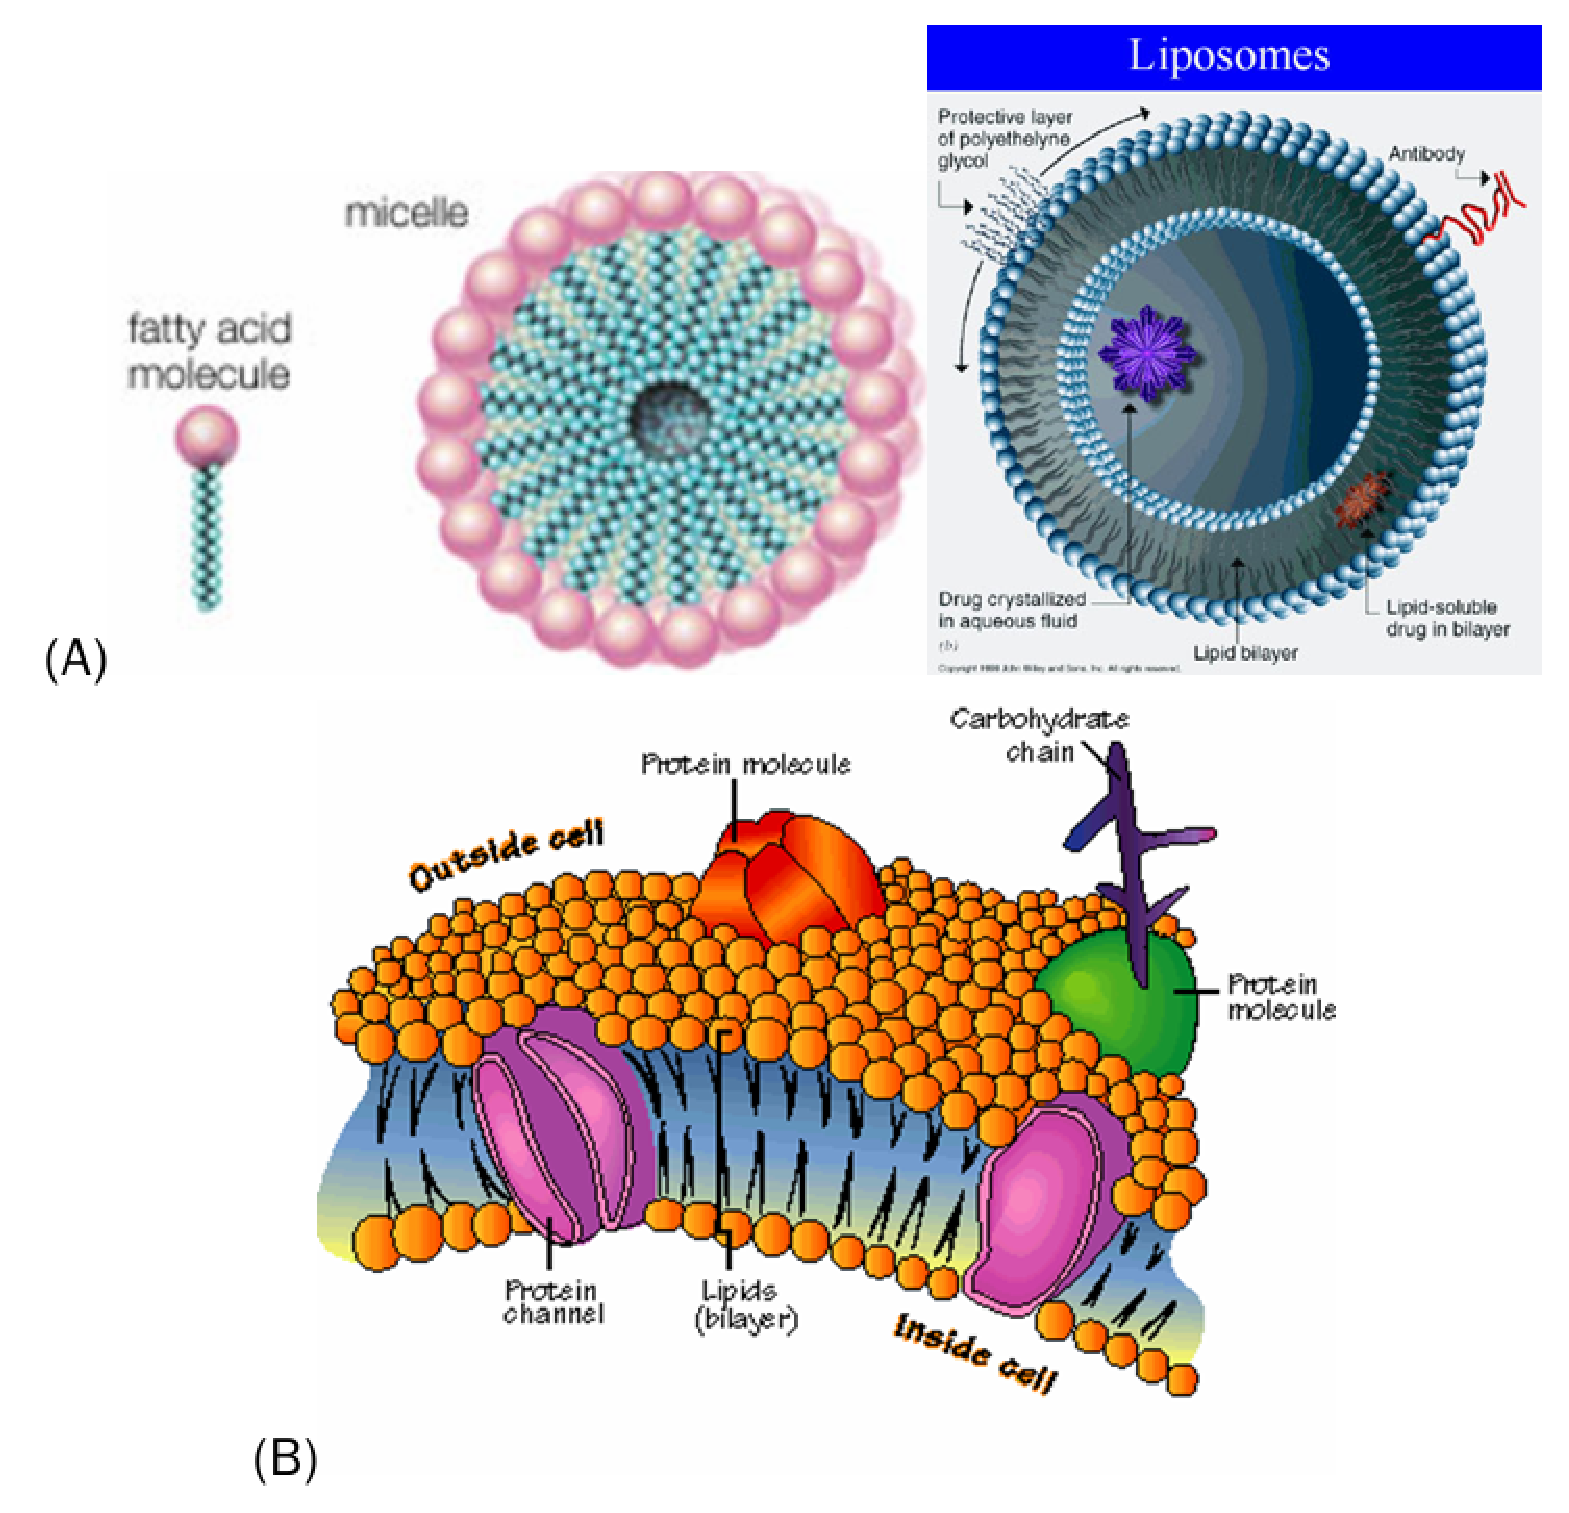
\includegraphics[height=5cm,
    angle=0]{./images/lipid_layers.eps}}
\caption{(A) spherical-like, (B) sheet-like}
\label{fig:lipids}
\end{figure}

\begin{figure}[hbt]
  \centerline{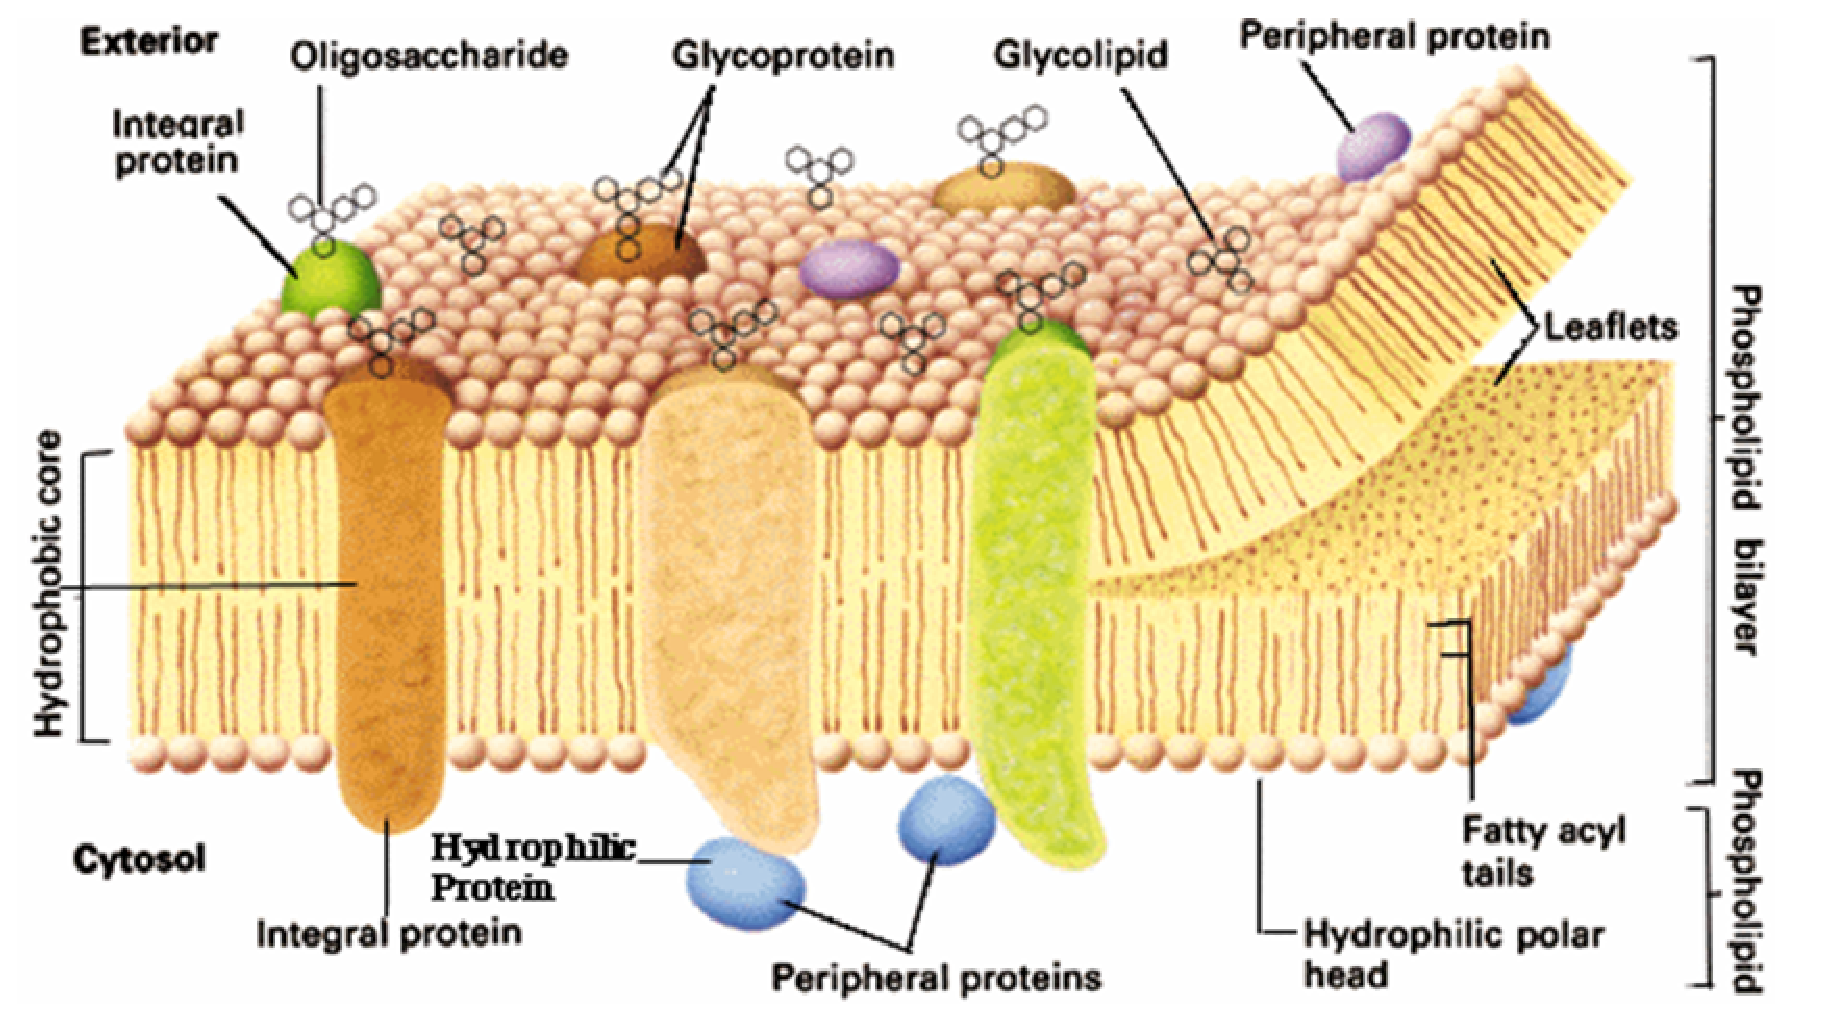
\includegraphics[height=5cm,
    angle=0]{./images/sheetlike_bilayer.eps}}
\caption{A sheet-like phospholipid bilayer in details}
\label{fig:sheet-like}
\end{figure}


\section{-- Lipids in cell membrane}
\label{sec:cell-membrane}

Lipids (Sect.\ref{sec:lipids}) are the essential components in a cell membrane,
with
\begin{itemize}
  
   \item {\bf phospholipids} (or {\bf phosphoglycerides}) are the principal
   building block of most biomembranes, with one polar head group and two
   non-polar (hydrophobic) tails.

When the phospholipids are mechanically dispersed in aqueous solution,
the phospholipids aggregate into one of three forms:
{\it spherical micelles}, liposomes, and
{\it sheetlike phospholipid bilayers}. In any configuration, the
hydrophobic ``tails" allign themselves tightly together in the center
to minimize their interaction with water. 
So the cell membrane is often bilayer.
Each phospholipid layer in this lamellar structure is called a leaflet. There
are three important properties of the bilayers:
\begin{enumerate}
\item The hydrophobic core is impermeable barrier that prevent the
  diffusion of water-soluble solutes. However, to allow some specific
  to go through, there are membrane tranport proteins embeded in the
  plasma membrane.
\item Its stability: the bilayer structure is maintained by
  hydrophobic and Van der Waals interactions between lipid chains.
\item All phospholipid bilayers can spontaneously form sealed closed
  compartments

\end{enumerate}

   \item The other principal classes of membrane lipids are {\bf sphingolipids}
   and {\bf cholesterol} (Sect.\ref{sec:cholesterol}). They are amphipathic.

The sphingolipids include the sphingomyelins and glycosphingolipids (the
cerebrosides, sulfatides, globosides and gangliosides). Sphingomyelins are the
only sphingolipid that are phospholipids. 
\end{itemize}

Because exposure the edges of the bilayer to solvent is highly
unfavorable, extensive bilayers normally wrap around themselves and
form closed versicles, i.e. all cell membranes enclose an entire cell.
As a result, cells have an {\it internal face} and an external face
(the surface presented toward the extracellular environment). More
commonly, we designate the two surfaces as the {\bf cytosolic surface}
and {\bf exoplasmic face}, correspondingly.  
\begin{figure}[hbt]
  \centerline{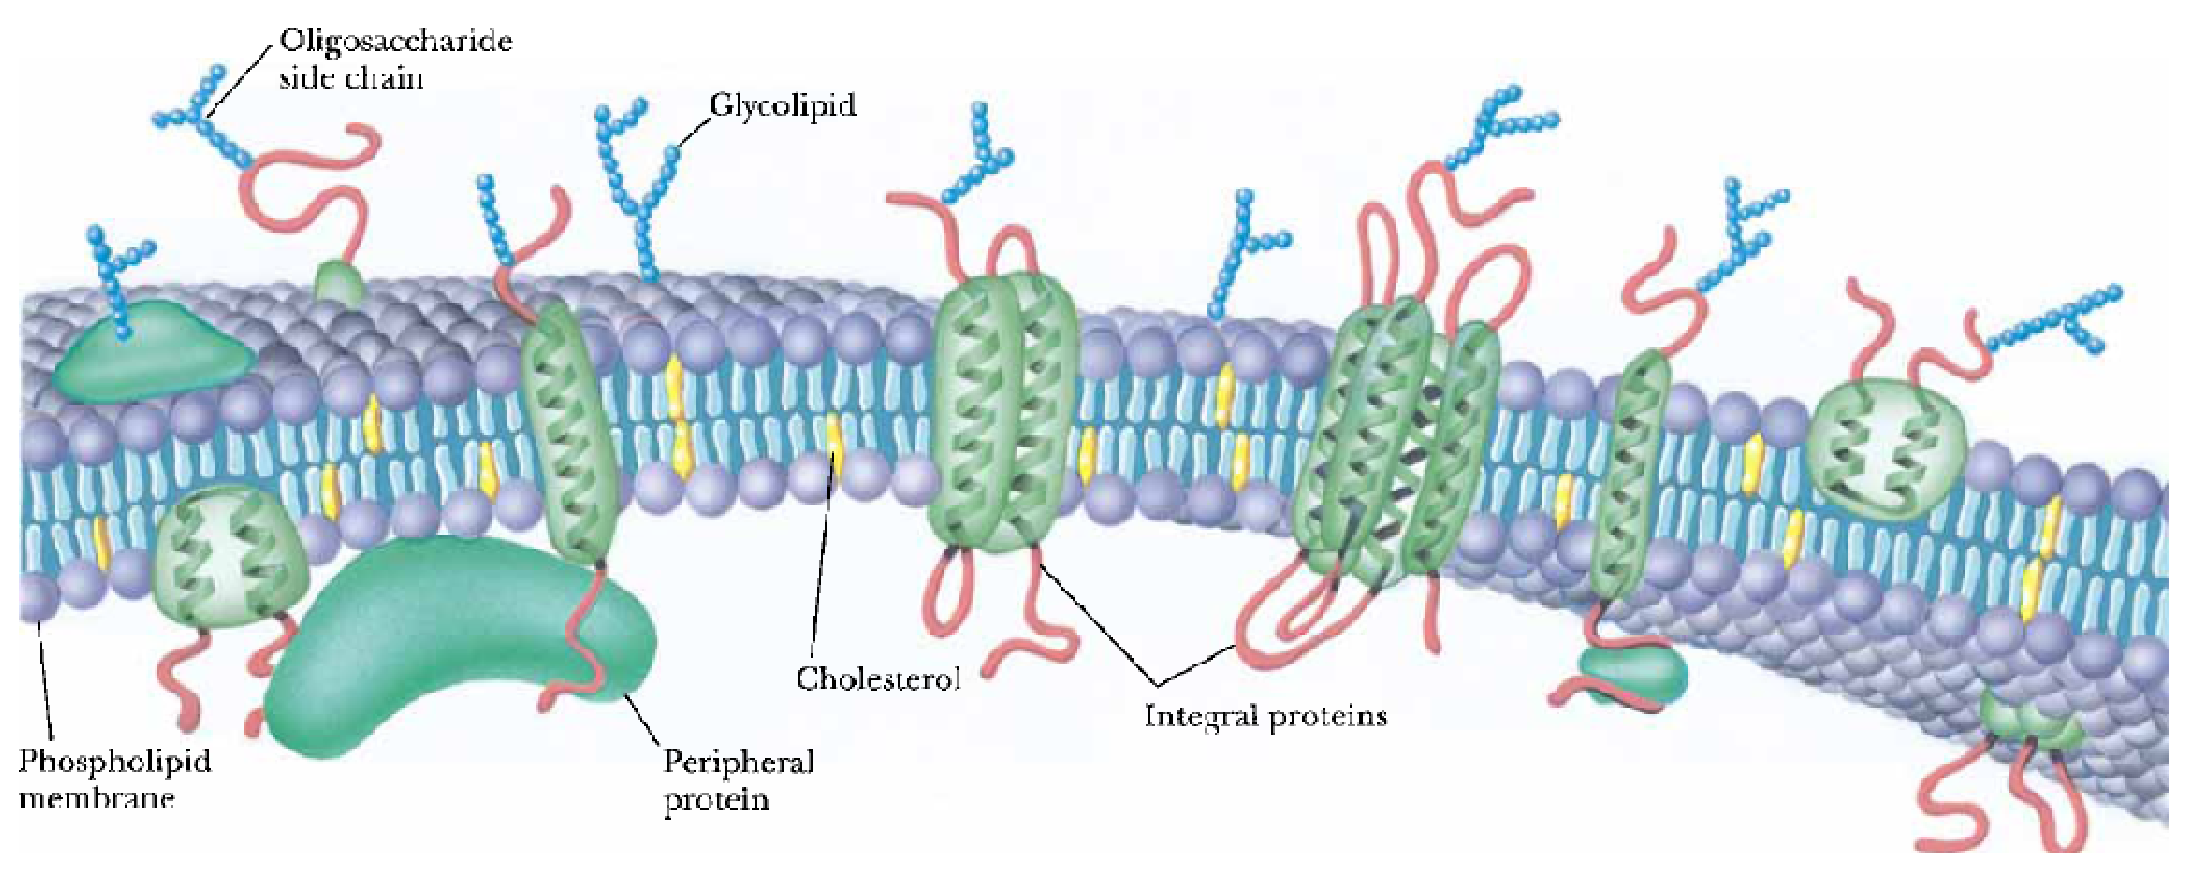
\includegraphics[height=5cm,
    angle=0]{./images/mosaic_model.eps}}
 \caption{Fluid Mosaic model}
\label{fig:mosaic_fluid}
\end{figure}

\section{-- Lipid in waters}
\label{sec:lipid-in-water}

The chemical potential (i.e. speed of reaction) of a hydrocarbon in
water is given
\begin{equation}
  \mu_{HC,wat} = \mu_{HC,wat}^0 + RT \ln(f_{HC,wat}\times X_{HC,wat})
\end{equation}
with $f$ is the coefficient of chemical activity and $X_{HC,wat}$ is
the concentration (or mole fraction). HC is the hydrocarbon that,
in this case, is lipid. So we can rewrite the equation
\begin{equation}
  \mu_{lip,wat} = \mu_{lip,wat}^0 + RT \ln(f_{lip,wat}\times X_{lip,wat})
\end{equation}

In water environment, solubility of HC is very low, then the mutual
interaction of HC is negligible, or $f \approx 1$. 
In a hydrocarbon environment (HC-HC), we also have
$X_{lip, HC} = 1$.
\begin{equation}
  \mu_{lip,HC} = \mu_{lip,HC}^0 + RT \ln(f_{lip,HC}\times X_{lip,HC})
\end{equation}
When the equilibrium is hold, the chemical potential will then be
equal $\mu_{lip,wat} = \mu_{lip,HC}$. Also, for simplicity, we assume
$f_{lip,HC} = 1$, then
\begin{equation}
  \mu_{lip,BL}^0 = \mu_{lip,wat}^0 + RT \ln X_{lip,wat}
\end{equation}

Based on experimental data, C. McAuliffe stated that
\begin{equation}
  \ln X_{lip,wat} = -4.11 - 1.49 n_C
\end{equation}
with $n_C$ is the number of carbons in the chain. It means that  the
energy increase $0.006aJ$ for each additional methyl group (\ce{CH3-})
in the hydrocarbon chain. Adding one lipid to the BL
\begin{equation}
  \label{eq:1}\begin{split}
  \Delta \ln X_{lip,wat}& = (-4.11) - 1.49 (n_c+1)-(-4.11-1.49n_c)\\
&= -1.5 \\
RT\Delta \ln X_{lip,wat} &=-1.5RT = -1.5\times 2.4 kJ/mol \\
&\approx -3.6 kJ/mol
\end{split}
\end{equation}


If we want to examine whether a lipid prefer to stay in aqueous
environment or in the bilayer, we cannot assume $X_{lip,HC} = 1$,
since in a bilayer, there can be different types of lipids
(i.e. HC). A general form 
\begin{equation}
  \mu_{lip,BL} = \mu_{lip,BL}^0 + RT \ln(f_{lip,BL}\times X_{lip,BL})
\end{equation}

Here, we deals with two states of lipids: join with bilayer or aqueous
environment. In practice, the situation is more complicated, there are
different states of aggregation in which a lipid can participate. 

\section{-- Micelles}
\label{sec:lipid-in-micelle}
\label{sec:micelle}

\begin{equation}
  \label{eq:2}\begin{split}
  \mu_{lip,wat}& = \mu_{lip,mi} \\
  \mu_{lip,mi} &= \mu_{lip,mi}^0+\frac{RT}{m}\ln (X_{lip,m}/m) \\
\end{split}
\end{equation}
with $m$ is the number of lipids in the micelles.

In the two environments:

\begin{equation}
  \label{eq:3}
  X_{lip,mi} = m \times X_{lip,w}^m \exp (-\frac{m}{RT}(\mu_{lip,mi}^0-\mu_{lip,wat}^0))
\end{equation}
Based on this equation, we notices that:
\begin{itemize}
\item $X_{lip,mi}$ is monotonic with $X_{lip,wat}$
\item $X_{lip,mi}$ decrease with m as
  $(\mu_{lip,mi}^0>\mu_{lip,wat}^0)$

NOTE: $X_{lip}$ always less than 1
\item $X_{lip,mi}$ increase with m.
\end{itemize}

Regarding surface effects, bear in mind that the negatively charged
outer surface of a phospholipid bilayer will attract protons, and
this produces a local change in pH, as follows
\begin{equation}
  \label{eq:13}
  pH_{surface} = pH_{bulk} + \frac{q_e\Psi_0}{2.3k_BT}
\end{equation}
where $q_e = 1.6\times 10^{-19} C$ is electronic charge, and $\Psi_0$
is the surface potential.
\section{The synthesis of phospholipids and cholesterols}
\label{sec:synth-phosph-chol}
\label{sec:cholesterls}

Finally, we consider how phospholids and cholesterol are synthesized
in cells and distributed to the many membranes and organelles.

\section{Phospholipids}
\label{sec:phospholipids}

STRUCTURE:
\begin{itemize}
  \item a head: hydrophilic group consisting a phosphate group
  
  \item two tails: hydrophobic groups
\end{itemize}
\begin{verbatim}
      ------------tail1 (R1)
head-<
      ------------tail2 (R2)
\end{verbatim}
Within these three classes of membrane lipids
(Sect.\ref{sec:phospholipid-classification}), enormous diversity results from
various combinations of fatty acid "tails" and polar "heads."

Phospholipids is the major component of cell membranes; besides other molecules
(e.g., proteins, glycolipids, sterols). Phospholipids are organized in a
bilayer, when hydrophobic tails line up against one another.
\begin{verbatim}
   head head ...
   /\   /\
  | |  | |
 T1 T2
 T1 T2
  | |  | |  ...
  \/   \/
  head head ...
\end{verbatim}

The phospholipid molecules are hypothesized to act as a solvent for all the
substances and proteins within it, i.e. the (transmembrane) proteins and
glycolipids are free to diffuse laterally through the lipid matrix and migrate
over the membrane. Sterols contribute to membrane fluidity by hindering the
packing together of phospholipids.

\subsection{-- classification}
\label{sec:phospholipid-classification}

Three general types of membrane lipids, Fig.\ref{fig:phospholipids}
\begin{enumerate}
  \item {\bf glycerophospholipids}:  two fatty acids joined to glycerol -
  Sect.\ref{sec:glycerol}
  
  \item {\bf sphingolipids}: a single fatty acid is joined to a fatty amine,
  sphingosine
  
  \item {\bf sterols}: a rigid system of four fused hydrocarbon rings
\end{enumerate}

Glycerophospholipids and sphingolipids contain polar or charged alcohols at
their polar ends; some also contain phosphate groups.

\begin{figure}[hbt]
  \centerline{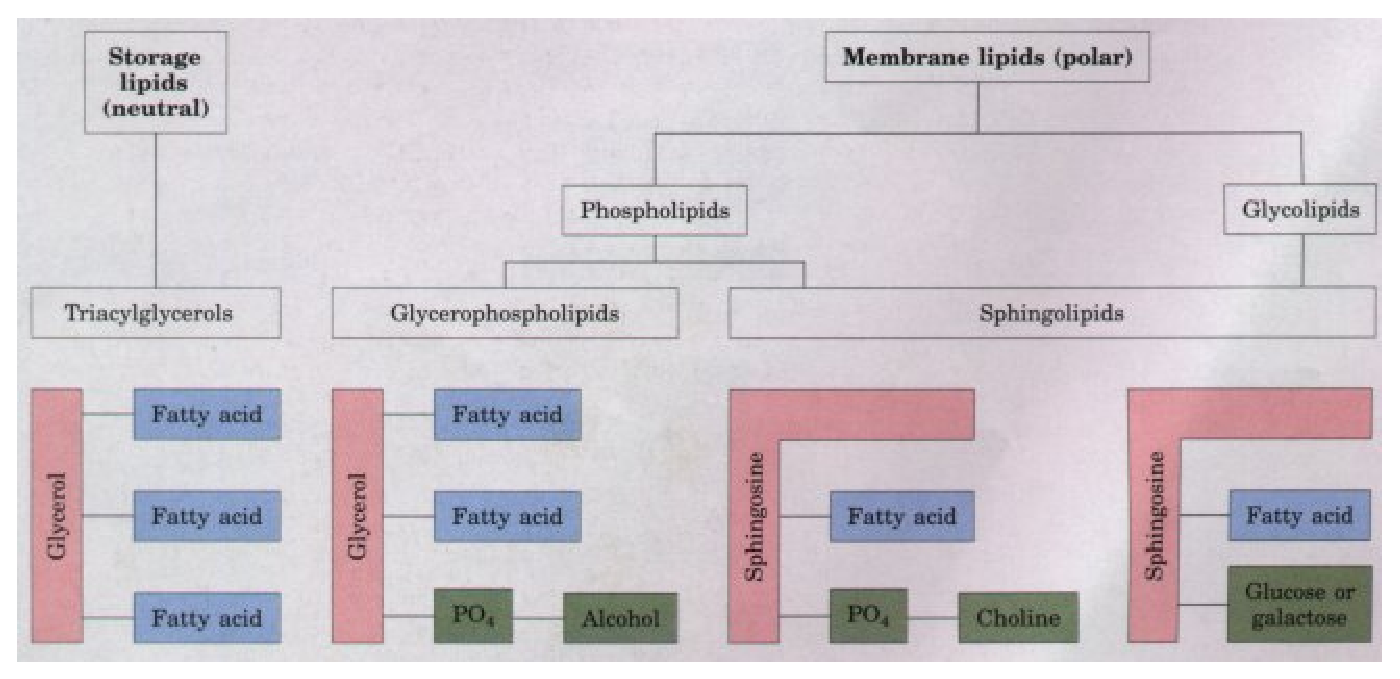
\includegraphics[height=3cm,
    angle=0]{./images/phospholipids.eps}}
\caption{Storage lipids and membrane lipids}
%http://www.bioinfo.org.cn/book/biochemistry/chapt09/bio2.htm
\label{fig:phospholipids}
\end{figure}


\subsection{-- function as signal transduction}

Some  types of phospholipid can be split to produce products that function as
second messengers in signal transduction
\begin{enumerate}
  \item PIP2 - Sect.\ref{sec:PIP2}: activated PLC split PIP2 into IP3 (free) and
  DAG (membrane-bound)
  
  \item 
\end{enumerate}

\subsection{Glycerophospholipid (phosphoglycerides)}
\label{sec:glycerophospholipid}
\label{sec:phosphoglycerides}

{\bf Glycerophospholipids} (or phosphoglycerides) are glycerol-based
phospholipids (Sect.\ref{sec:phospholipids}), and is the most abundant of the
polar lipids in most membranes. The formation of glycerophospholipid is
discussed in Sect.\ref{sec:glycerol}.

Each glycerophospholipid has:
\begin{itemize}
  \item head with glycerol as the backbone 
  
\begin{verbatim}
CH2- R1
|
CH-  R2
|
CH2- PO4- X 

NOTE: X = head-group-substituent
\end{verbatim}
with C1- and C2- connecting two tails; and C3- attached to a highly polar or
charged (and therefore hydrophilic) head group through phosphodiester bond. 
  
  \item two tails as {\it non-polar fatty acid regions}:
  hydrocarbon tails of fatty acids, designated R1, R2, with ester linking to
  C1- and C2- of glycerol.
\end{itemize}


All glycerophospholipids are named for their polar head group
\begin{enumerate}
  \item Phosphatidylinositol (PI) - Sect.\ref{sec:phosphatidylinositol}
  \item Phosphatidylcholine (PC) - Sect.\ref{sec:phosphatidylcholine}
  \item Phosphatidylglycerol (PG) - Sect.\ref{sec:phosphatidylglycerol}
  \item Glycosyl phosphatidylinositols (GPI) - Sect.\ref{sec:GPI}
\end{enumerate}
All have a negative charge on the phosphate group at pH 7.0. The head-group
alcohol may also contribute one or more charges at pH near 7.
\footnote{\url{https://www.rpi.edu/dept/bcbp/molbiochem/MBWeb/mb1/part2/lipid.htm}}

{\it Neural membranes} contain several classes of glycerophospholipids which
turnover at different rates with respect to their structure and localization in
different cells and membranes.


  
\subsection{1. phosphatidylcholine (PC)}
\label{sec:phosphatidylcholine}

Phosphatidylcholine is a class of phospholipid with choline as the head-group.
\begin{equation}
\text{Choline} = \ce{-CH2-CH2-N^+(CH3)_3}
\end{equation}
Phosphatidylcholine (PC) is one of the 4 main components of the cellular plasma
membrane (Sect.\ref{sec:glycerophospholipid}).
PC is more commonly found in the exoplasmic or outer leaflet of a cell membrane.
It is thought to be transported between membranes within the cell by
phosphatidylcholine transfer protein (PCTP). PC also plays a
role in membrane-mediated cell signaling and PCTP activation of other enzymes.
 
Phospholipase D (Sect.\ref{sec:PLD}) catalyzes the hydrolysis of
phosphatidylcholine to form phosphatidic acid (PA), releasing the soluble
choline headgroup into the cytosol.

Arachidonic acid-containing phosphatidylcholine (AA-PC), [PC(16:0/20:4)+K]+
\begin{itemize}
  \item  significantly increased in the ipsilateral ventral and dorsal horns of
  the spinal cord after sciatic nerve transection in PNI (Sect.\ref{sec:PNI})
\end{itemize}

\subsection{2. phosphatidylglycerol (PG)}
\label{sec:phosphatidylglycerol}

\begin{equation}
\text{Glycerol} = \ce{-CH2-CH(OH)-CH2-OH}
\end{equation}

\subsection{3. glycosyl phosphatidylinositol (GPI)}
\label{sec:GPI}
\label{sec:glycosyl-phosphatidylinositol}

Glycosyl phosphatidylinositol (GPI or glycosyl-PI) is complex glycolipids that
is the predominant form of membrane-attachment, i.e. attach some proteins to the
{\it outer surface} of the plasma membrane (Homans et al., 1988).


\subsection{4. Phosphatidylinositol (PI, PtdIns)}
\label{sec:phosphatidylinositol}

{\bf Phosphatidylinositol} (PtdIns, PI) is classified as glycerophospholipids
(Sect.\ref{sec:glycerophospholipid}).

\begin{equation}
\text{myo-Inositol = a six-carbon ring} 
\end{equation}
NOTE: In the phosphorylate forms of PI (to be discussed later), one or many
hydroxyl group (-OH) in the myo-inositol polar ring (Sect.\ref{sec:inositol})
will be substituted with phosphate groups by the enzyme phosphatidilinositol
synthase (PIS).

\begin{figure}[hbt]
  \centerline{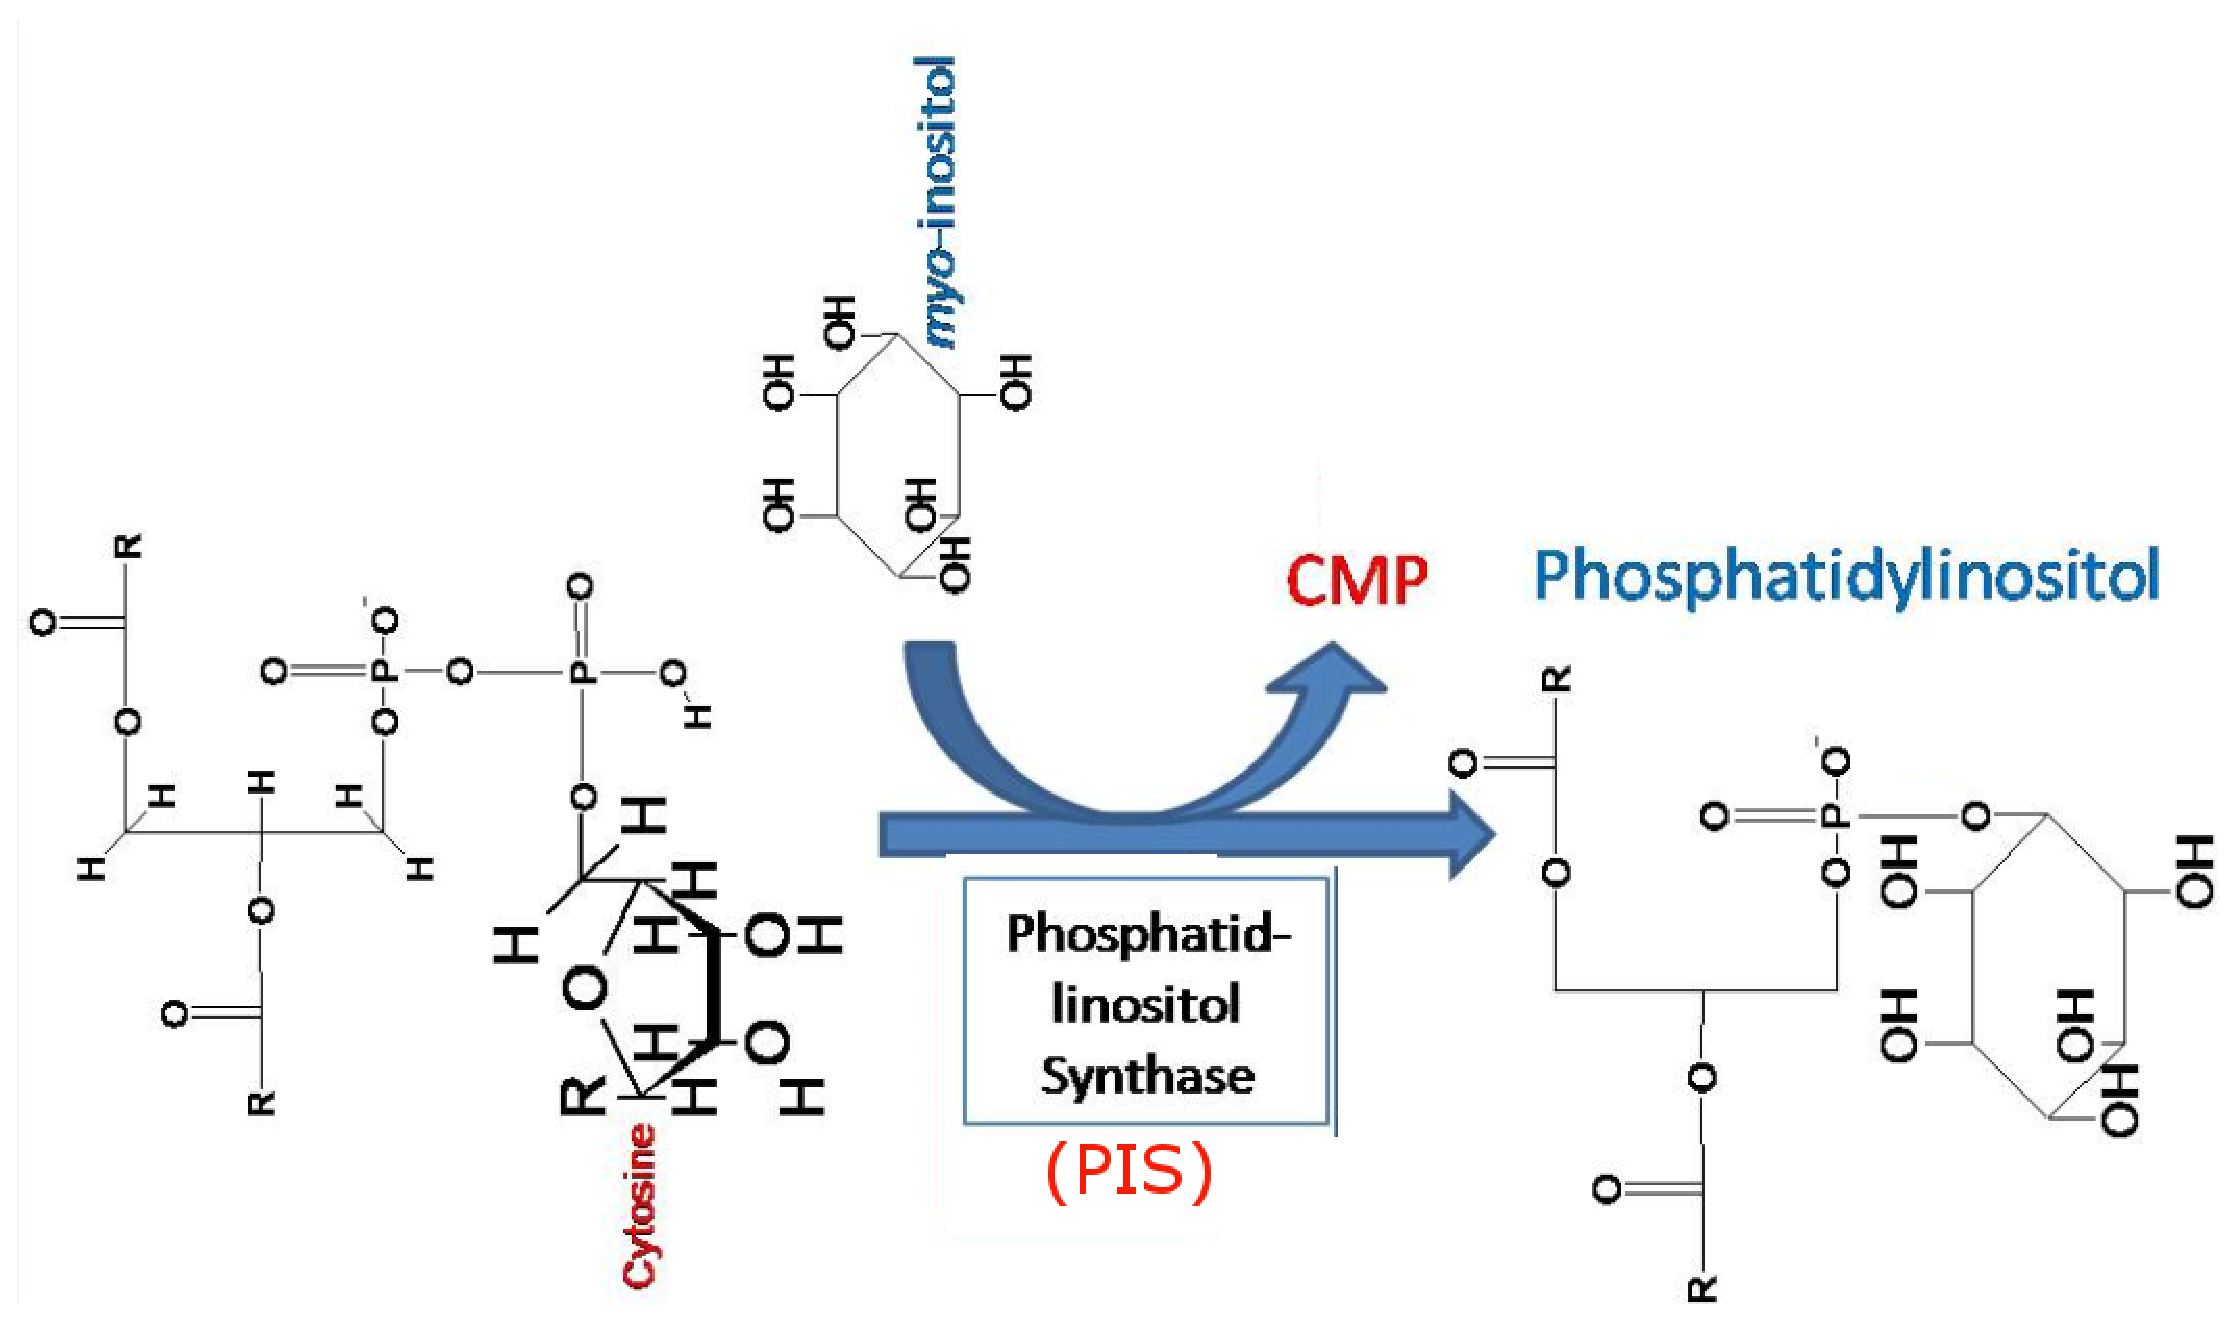
\includegraphics[height=5cm,
    angle=0]{./images/PtdIns-biosynthesis.eps}}
  \caption{PtdIns biosynthesis}
  \label{fig:PtdIns-biosynthesis}
\end{figure}

\textcolor{red}{\bf SYNTHESIS MECHANISM}: PI is synthesized by a single enzyme
called {\bf phosphatidylinositol synthase} (PIS) which uses myo-inositol and
cytidine-diphosphate (CDP)-diacylglycero as substrates; the second product is
produce cytidine-monophosphate (CMP), Fig.\ref{fig:PtdIns-biosynthesis}

\begin{verbatim}
myo-inositol + cytidine-diphosphate (CDP)-diacylglycero
       ---(enzyme: PIS)-------> PI +  CMP
\end{verbatim}

\begin{mdframed}

{\bf SYNTHESIS LOCATION}: Not only on ER membrane; but also other membrane
locations, including plasma membrane.

As PIS is an integral membrane protein of the endoplasmic reticulum (ER) which
is required to synthesize PI, it has been believed that PI is synthesized in the
ER before being moved to the plasma membrane with the help of PI-transfer proteins (PITP),
Fig.\ref{fig:PtdIns-mobilization}(A). However, recent evidences challenge this
dogma by showing that under {\bf phosphatidylinositol depletion}, to help
quickly producing PI, {\bf Sar1 GTPase-dependent cycle} can create a mobile
PI-producing compartment that transport PIS from the ER to numerous cellular
compartments, including the plasma membrane, to produce PI
Fig.\ref{fig:PtdIns-mobilization}(B) \citep{kim2001, bankaitis2001}.
\end{mdframed}
% with \begin{itemize} \item PIS-containing mobile vesicle compartment \item
% Diacylglycerol-containing mobile vesicular compartment \end{itemize} and

\begin{figure}[hbt]
  \centerline{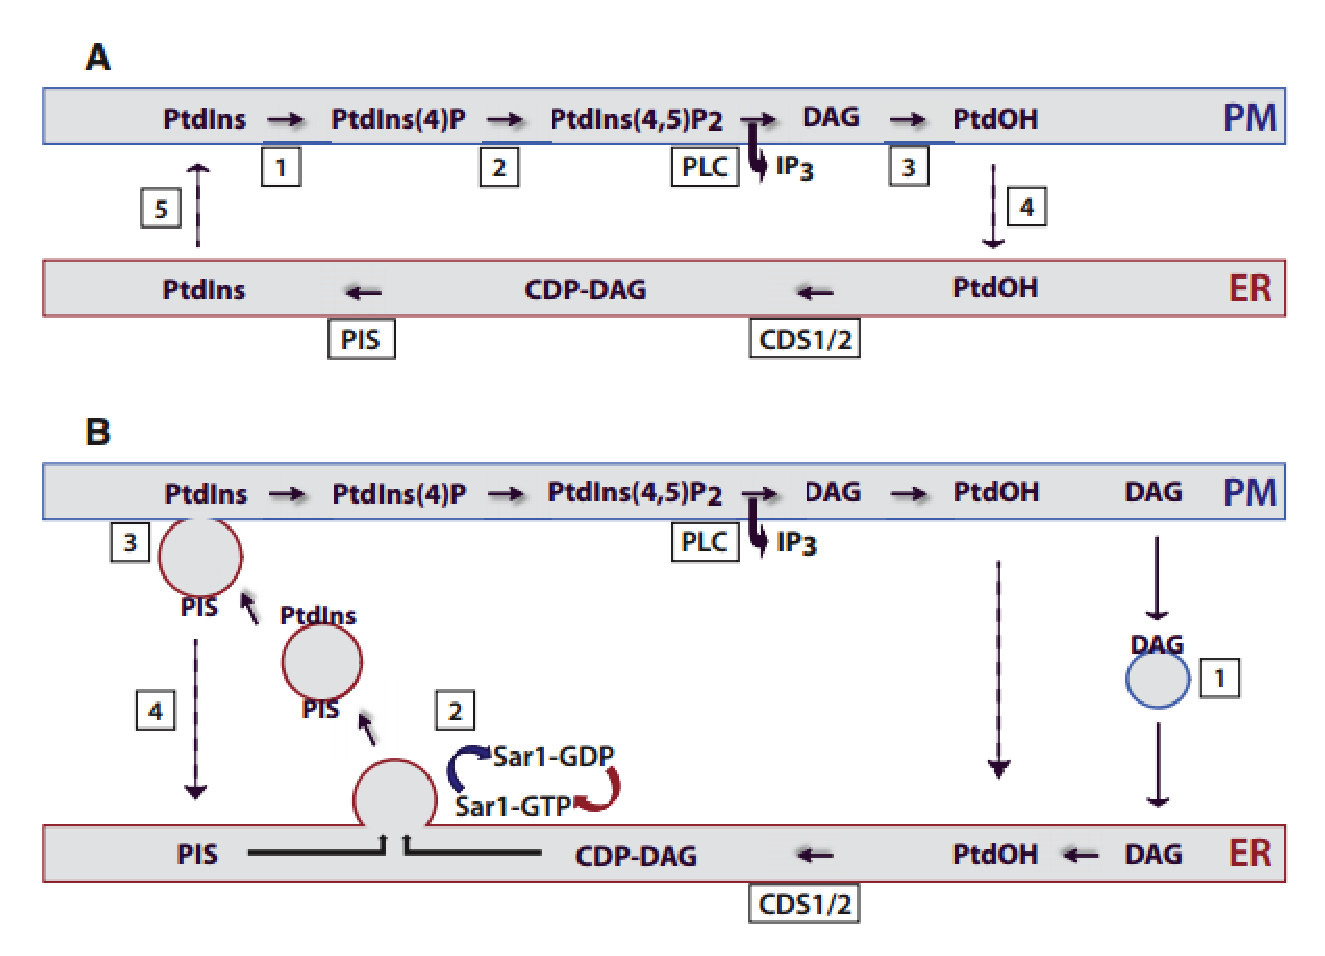
\includegraphics[height=7cm,
    angle=0]{./images/PtdIns-mobilization.eps}}
  \caption{(A) PI is produced in the ER membrane, then migrate to
  plasma-membrane where (1) PI is phosphorylated by 4-OH kinase into PI(4)P, and
  then (2) PI(4)P phosphorylated by 4-phosphate 5-OH kinase to generate
  PIP2; (B) PI is produced directly in the plasma-membrane as PIS is
  delivered to the plasma-membrane by Sar1 GTPase-dependent cycle
  which cooperates with PIS to produce a mobile compartment containing PI and
  PIS to deliver to the membrane \citep{bankaitis2001}}
  \label{fig:PtdIns-mobilization}
\end{figure}


PI integrates multiple intracellular signaling pathways and thus modulate a
large range of cellular activities. Its role is reflected via its different
phosphorylated forms, such as PIP2 (Sect.\ref{sec:PIP2}) and PIP3
(Sect.\ref{sec:PIP3}). The phosphorylated forms of PtdIns are called {\it
phosphoinositides} or (if two or more phosphpate groups are replaced) {\it
polyphosphoinositides} (PPI) (Sect.\ref{sec:phosphoinositides}).

\subsection{-- localization}
\label{sec:PtdIns-localization}
\label{sec:PI-localization}

The localization of PI is also considered important which is thought to provide
essential spatial and temporal cues for protein recruitment and intracellular
membrane traficking.

\textcolor{red}{\bf LOCALIZATION}: PI
\begin{enumerate}
  
  \item presynaptic side: the turnover of PI is critical for neurotransmitter
  vesicle cycling and synaptic function
  
  \item postsynaptic side:
\end{enumerate}


%  consists of a family of structural
% lipids (on cell membrane) with myo-inositol is an important component - the polar head group . 
\subsection{-- Phosphoinositides and Polyphosphoinositides (PPI)}
\label{sec:phosphoinositides}
\label{sec:polyphosphoinositides}
\label{sec:PPI}

The phosphorylated forms of PtdIns (Sect.\ref{sec:phosphatidylinositol}) are
called {\it phosphoinositides} which play an important role in cell signaling,
membrane trafficking. There are different names, depending on the number of
phosphate groups being substituted. 
The myo-inositol ring of the PtdIns can be phosphorylated at position 3, 4, and
5, Fig.\ref{fig:PtdIns-biosynthesis}. The two and six hydroxyl group is
typically not phosphorylated due to steric hindrance (i.e. higher energy price,
slow reaction rate).

\begin{itemize}
  \item {\bf phosphatidylinositol monophosphate}

Phosphatidylinositol monophosphates: there are 3 cases
  \begin{enumerate}
    \item PI(3)P: Phosphatidylinositol 3-phosphate, or PtdIns3P
    \item PI(4)P
    \item PI(5)P
  \end{enumerate}
  
  
  \item {\bf phosphatidylinositol bisphosphate}

Phosphatidylinositol biphosphates: there are 3 cases
  \begin{enumerate}
    \item PI(3,4)P2
    \item PI(3,5)P2
    \item PI(4,5)P2 = {\bf PIP2} = Phosphatidylinositol 4,5-bisphosphate -
    Sect.\ref{sec:PIP2}
  \end{enumerate}

 
  \item {\bf Phosphatidylinositol triphosphates (PIP3)}: there is 1 case:
  PIP3 = PI(3,4,5)P$_3$ = Phosphatidylinositol 3,4,5-trisphosphate

Only PIP3 is not found in plant cells.  
  
%   if there are are phosphorylated
%   derivatives of phosphatidylinositol (PtdIns) implicated in many aspects of cell function.
\end{itemize} 


\url{http://en.wikipedia.org/wiki/Phosphatidylinositol}

\begin{figure}[htb]
    \centerline{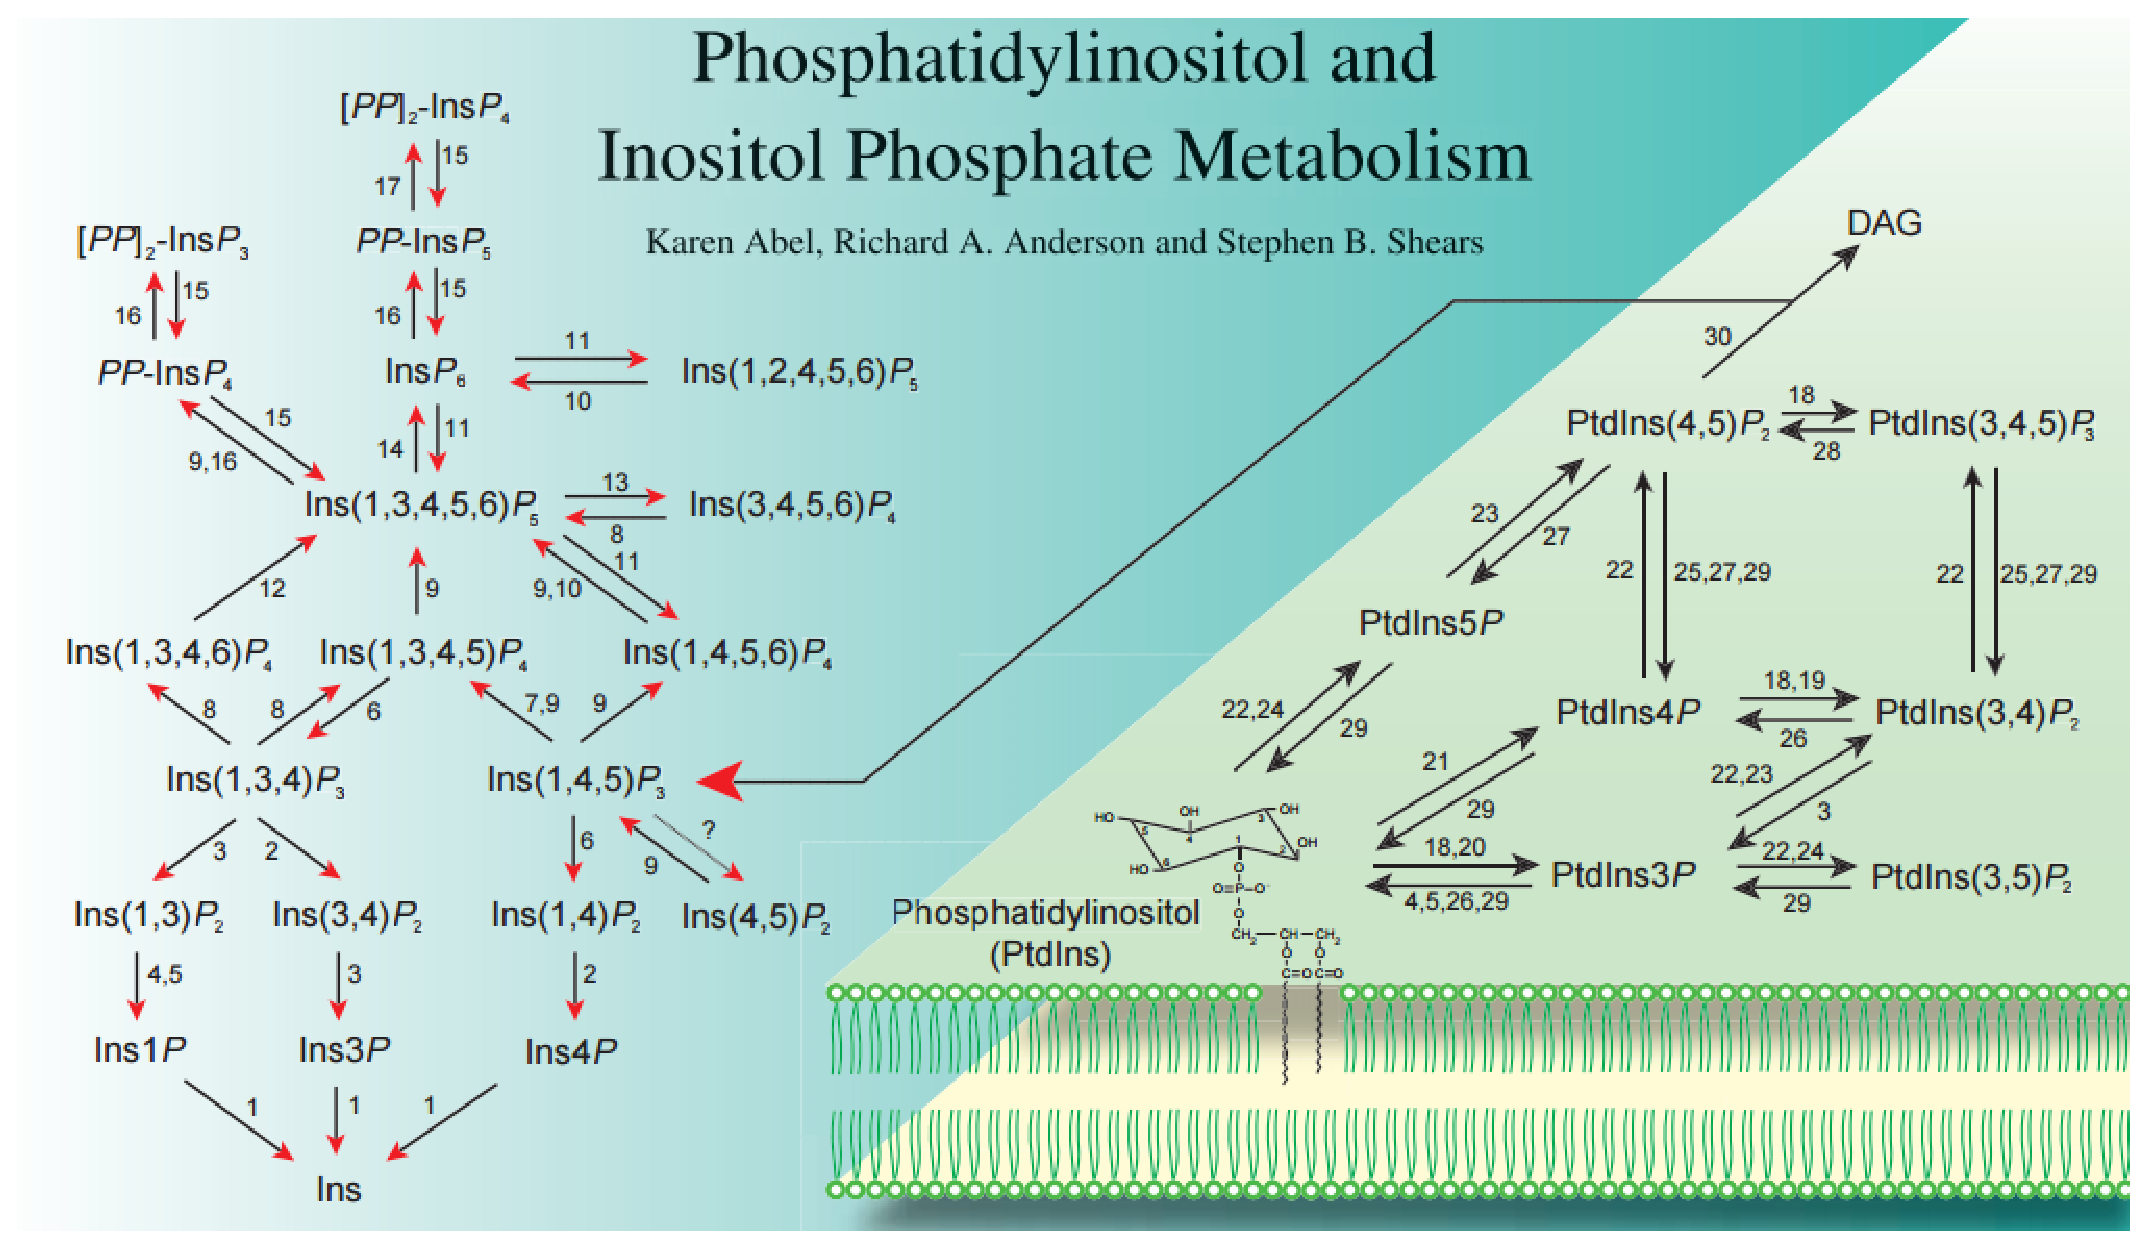
\includegraphics[height=9cm]{./images/Phosphatidylinositol-metabolism.eps}}
\caption{At (30): PIP2 is }\label{fig:Phosphatidylinositol-metabolism}
  \end{figure}


\subsection{-- PPI}

{\bf Polyphosphoinositides} (PPI) refers to the molecules when two (P(3,4)P2,
P(4,5)P2, P(3,5)P2) or three (PIP3) phosphate groups are replaced in
phosphoinositides (Sect.\ref{sec:phosphoinositides}). Among them, PIP2 is the
major isoform on the cell membrane of mammalian cells (Sect.\ref{sec:PIP2}).

\subsection{---- PIP2 (i.e. PI(4,5)P2)}
\label{sec:PIP2}

Other names: {\bf Phosphatidylinositol 4,5-bisphosphate} (or
4,5-biphosphatidylinositol), abbreviated as PtdIns(4,5)P2, or PI(4,5)P2.

Though PIP2 is a minor phospholipid component of cell membrane (about $1\%$ of
total anionic phospholipids), PIP2 is the major form of PPI
(Sect.\ref{sec:polyphosphoinositides}) on the cell membrane of mammalian cells
(review: \citep{McLaughlin2002}), and once phosphorylated it becomes PIP3
(Sect.\ref{sec:PIP3}).


\textcolor{red}{SYNTHESIS MECHANISM}: PIP2 is synthesized from the
phosphorylation of PI(4)P (Sect.\ref{sec:phosphatidylinositol}) by PI(4)P 5
kinase (i.e. 4-phosphate 5-OH kinase, Fig.\ref{fig:PtdIns-mobilization}(A));
upon the activation of PI(4)P 5 kinase by phosphatic acid (PA).
NOTE: PA is the product of phospholipase D, and the small GTPase Arf.

NOTE: small GTPase Arf also activate PI4 kinase.

\begin{verbatim}
PtdIns (or PI) 
   --phosphorylated by 4-OH kinase-> PI(4)P 
        ---phosphorylated 4-phosphate 5-OH kinase--> PI(4,5)P (or PIP2) 
\end{verbatim}

\begin{mdframed}
PIP2 is important in the attachment of the cytoskeleton to the plasma membrane,
exocytosis, endocytosis, membrane trafficking, and the activation of enzyme. 

\textcolor{red}{A cytosolic protein with charges no less than 12 charges is
needed for it to bind PIP2 or PIP3.}

\textcolor{red}{How can a single lipid PIP2 can have so many role?} -

SUGGESTION: there are different pools of PIP2 in the plasma membrane, i.e.
non-uniform distribution of PIP2 on plasma membrane, which makes it possible to
function as spatial and temporal detector/transducer for signal.

\end{mdframed}

PIP2 can be 
\begin{enumerate}
  \item converted to PIP3 by PI3K - Sect.\ref{sec:PIP3}
  
  \item hydrolyzed by PLC-$\beta$ to produce DAG and IP3
  (Sect.\ref{sec:GPCR-PLC-IP3-DAG-pathway}),
  Fig.\ref{fig:Phosphatidylinositol-metabolism}. 

\begin{Verbatim}
      hydrolyzed by PLC-beta 
PIP2 -----------------------> IP3 + DAG
\end{Verbatim}

\end{enumerate}




\subsection{---- PIP3 (i.e. PI(3,4,5)P3)}
\label{sec:PIP3}

PIP3 is the maximal phosphorylated form (i.e. P(3,4,5)P3) of phosphoinositides
from PIP2 (Sect.\ref{sec:PIP2}) by PI3K (Sect.\ref{sec:PI3K}).
PIP3 is phosphorylated by phosphoinositide 3-kinase (PI3K) -
Sect.\ref{sec:PI3K}.
\begin{equation}
\ce{PIP2 <=>[PI3K][PTEN] PIP3}
\end{equation}

PIP3 is trisphosphorylated, and therefore has the potential to exhibit complex ionization
behavior. Each of the phosphates in the head group have the ability to titrate independently of
each other, but they also have the potential to interact with each other due to their close
proximity. 

PIP3 is the most difficult to characterize PI, due to its low basal abundance.
To test the role of PIP3, a domain with high-specificity to PIP3 was used to
remove the availability of PIP3 for binding with other endogenous targets on CA3
neuron. PIP2 exhibits complex ionization behavior and shares a similar structure
to PIP3. It was believed that the 4 and 5 phosphate of PIP3 would also exhibit
complex ionization behavior, but it was not known how the presence of the 3
phosphate group would affect this.


\begin{itemize}
  \item Sect.\ref{sec:synaptic-plasticity-CA3-to-CA1}

Overexpressing pleckstrin homology (PH) domain from General Receptor
for Phosphoinositides (GRP1) in CA1 neurons from organotypic hippocampal slice
cultures - such domain has 650-fold specificity to PIP3 than PIP2 and other
phosphoinosidites (Sect.\ref{sec:phosphoinositides}).

By affecting only CA1 cells; but not CA3 cells, it ensures recombinant proteins
only expressed on postsynaptic side.
  
  \item 
\end{itemize}
\textcolor{red}{For a cytosolic protein to be able to bind to PIP2 or PIP3
directly; it needs to have the charge of no less than 12 charges.}

% Similar to PIP2, PIP3 can also be cleaved by PKC
% (Sect.\ref{sec:GPCR-PLC-IP3-DAG-pathway}), producing IP3 and DAG.

%(Sect.\ref{sec:phosphoinositides})

% \textcolor{red}{PIP3 is the phosphorylation from PIP2.} PIP3 is a phospholipid
% resides on the plasma membrane. 

\url{http://en.wikipedia.org/wiki/Phosphatidylinositol_(3,4,5)-trisphosphate}

\section{Diacylglycerol (DAG)}
\label{sec:DAG}
\label{sec:DAG_synthesis}

% {\bf diacyl glycerol} (DAG)
{\bf Diacylglycerol} (DAG, di-glyceride) is a membrane-bound glyceride (i.e. an
ester formed from glycerol and fatty acids). 

\begin{itemize}
  \item A glycerol has 3 hydroxyl functional groups which can be esterified with
  1, 2 or 3 fatty acids to form monoglyceride, diglyceride, or triglyceride.

Vegetable oils and animal fats contain mostly triglycerides, which can be broken
down into mono- or di- form.

  \item The two fatty acids in diglyceride can bind to either C-1 and C-2
  positions or the C-1 and C-3 positions.
  
\end{itemize}

There are two possible forms of DAG:
\begin{enumerate}
  \item 1,2-DAG
  
  \item 1,3-DAG
\end{enumerate}
NOTE: Remember that glycerol is the head-part of phosphatidylglycerol
(Sect.\ref{sec:phosphatidylglycerol}).

\textcolor{red}{DAG synthesis} is 
\begin{enumerate}

  \item Sect.\ref{sec:GPCR-PLC-IP3-DAG-pathway} which also produces IP3
  (Sect.\ref{sec:IP3}). However, IP3 is diffusible, but \textcolor{blue}{DAG
  remains bound to the membrane} (due to its hydrophobic property).

DAG formation is one of the two products of the hydrolysis of PIP2
(Sect.\ref{sec:PIP2}) by enzyme PLC-beta (Sect.\ref{sec:PLC}) - with the
co-factor of $\Ca$ for PLC to function; the other product of this process is
IP3.

\begin{verbatim}
PLC + [Ca2+] ----[cleave off IP3 group from phospholipid]----> DAG + IP3
\end{verbatim}

  \item hydrolysis of phosphatidylcholine (Sect.\ref{sec:phosphatidylcholine})

\begin{verbatim}
PC --[hydrolysis by PLC]---> DAG + phosphorylcholine

PC --[hydrolysis by PLD]--> phosphatic acid + choline
\end{verbatim}

Phosphatic acid and DAG are readily interconverted.

\end{enumerate}


DAG can 
\begin{enumerate}
  \item activate PKC (Sect.\ref{sec:PKC-activation})

DAG species vary in their ability to activate PKC.
  
  \item activate TRPC3, TRPC6, TRPC7 - a subfamily of transient receptor
  potential canonical (TRPC) cation channels (Sect.\ref{sec:TRPC})
  
\end{enumerate}




\section{Membrane proteins}
\label{sec:membrane-proteins}

The phospholipids constitute the fundamental structural unit of all biological
membranes. But it is the membrane proteins which carry out essentially all of
the active function of membranes.

In the Singer-Nicolson fluic mosaic model (Sect.\ref{sec:Singer-Nicolson}),
there are 2 types of proteins: peripheral proteins \& integral proteins. Another
class of proteins not anticipated by Singer and Nicolson is the lipid-anchored
proteins; these proteins associate with membranes by means of a variety of
covalently linked lipid anchors.

\subsection{-- integral proteins: unilateral + transmembrane}
\label{sec:transm-prot}
\label{sec:integral-proteins}

{\bf Integral membrane proteins} = glycoproteins: These proteins are
inserted into the plasma membrane so that the hydrophobic part is
surrounded by the hydrophobic portions of the lipids. These integral
membrane proteins are classified into 2 classes:
\begin{itemize}
\item {\it unilateral}: reaching only part way across the membrane

\item {\it transmembrane}: the two hydrophilic ends of the protein
  exposed on both sides of the membrane.
\end{itemize}


Transmembrane proteins have C-terminal end in the cytoplasm and
N-terminal (can be modified by various carbohydrates) extends over a
long distance into the outer environment of the cell).  These
carbohydrates, in some cases, functions as receptors and are location
of immunological reactions. Further, the N-terminal is where the
monomer of the N-acetylneuraminic acid (sialic acid) located. It
carries a dissociable carboxyl group. It means it carry a fixed
negative surface charges. Depending on cell types, there are 1-10
groups of sialic acid per 1nm$^2$ membrane area.  The glycoprotein
forms a loose external layer of the cell (glycocalyx = surface coat)
and the negative charges modify the thickness of the membrane
structure electrostatically.  The largest, oldest superfamily of
proteins that are transmembrane proteins: ATP-binding cassette
transporter
(ABC-transporter)\footnote{\url{http://en.wikipedia.org/wiki/ATP-binding\_cassette\_transporter}}.


\subsection{-- peripheral proteins}
\label{sec:peripheral-proteins}


{\bf Peripheral proteins} = cytoplasma protein: these proteins may be
(1) attached to integral proteins or (2) on the cytoplasmic side, they
are held by filaments of cytoskeleton. For the later situation, they
are parts of the cytoskeleton with connection to inner side of
membrane. 

Example, in human erythrocytes, they are heterodimeric protein with
molecular mass 260-220 kDa. They connect to each other by globular
actin molecular with molecular mass about 100 kDa.  Cytoskeleton is a
dynamic structure to control the lateral distribution of proteins in
the membrane.

\section{-- Proteins in lipid bilayer}
\label{sec:prot-lipid-bilay}

Protein exists in 2 states: r (relax) and t (expansion).
Let's consider an elementary layer with area of the cross-section is
$A(z)$ (relax) or $A_t(z)$ (expansion). 

The expansion of the protein would lead to the increase in the
energy. Then, it requires some work $W$ which can be due to pressure
$V=p(z)$. $W$ is the work done by a single molecule, then the total
work requires to multiply with an Avogadro number $N_A$.
\begin{equation}
  \label{eq:4}
  \begin{split}
    \mu_r &= \mu_r^0 + RT \ln[r] + W \\
\mu_t &= \mu_t^0 + RT ln[t]
  \end{split}
\end{equation}

Consider a reversible process: $r \leftrightarrows t$, at equilibrium,
we have $\mu_r = \mu_t$.

\begin{equation}
  \label{eq:5}
  \begin{split}
      dV_t(z) = A_t(z) dz \\
dV(z) = A(z) dz \\
ddV(z) = dV_t(z) - dVr(z)
  \end{split}
\end{equation}
Clearly, the change in volume leads to the change in work $\Delta W =
p dV$.

The work is now 
\begin{equation}
  \label{eq:6}
  W = N_A\int_Z p(z) ddV(z)
\mu_p^0 + RT \ln[r] + N_A\int(p(z).\Delta A.dz)
\end{equation}

Finally, 
\begin{equation}
  \label{eq:7}
  \mu_p^0 + RT ln[r]_0 + N_A\int p_0(z) \Delta A.dz = \mu_t^0 + RT\ln[t]_0
\end{equation}
with $p_0(z)$ is a new pressure. Then
\begin{equation}
  \label{eq:8}\begin{split}
  \mu_r^0 + RT\ln\frac{[r]}{[t]} + N_A \int p(z) \Delta A(z) dz =
  \mu_t^0 \\
  \mu_r^0 + RT\ln\frac{[r]_0}{[t]_0} + N_A \int p(z) \Delta A(z) dz =
  \mu_t^0 
\end{split}
\end{equation}

Next
\begin{equation}
  \label{eq:9}
  \begin{split}
    RT\ln \frac{[r]_0}{[t]_0} = -N_A \int \Delta p(z) \Delta A(z) dz
    \\
\frac{[r]}{[t]} = \frac{[r]_0}{[t]_0} .exp \left( -\frac{1}{k_BT}\int
  \Delta p(z) \Delta A(z) dz \right)
  \end{split}
\end{equation}

Finally, at p(z)
\begin{equation}
  \label{eq:10}
  F_t=\frac{[t]}{[r]+[t]} = \frac{1}{1+\frac{[r]}{[t]}}=\frac{1}{1+\frac{[r]_0}{[t]_0}e^\alpha}
\end{equation}
at $p_0(z)$
\begin{equation}
  \label{eq:11}
  F_{0,t} = \frac{[t]_0}{[r]_0+[t]_0} = \frac{1}{1+\frac{[r]_0}{[t]_0}}
\end{equation}
$\alpha$ depends on the fluctuation of the system. This ratio 
\begin{equation}
  \label{eq:12}
  f = \frac{F_t}{F_{0,t}}
\end{equation}
can be one state or another depending on...  this bilayer can actually
play important role in choosing the state of the protein.

SUMMARY:
\begin{itemize}
\item Bilayer is not simply the medium for protein to embed. It also
  effect the nature conformation of the embedded proteins.
\item State with lower energy (native state) also depend on the
  external environment, beside the chemical binding between its
  elements.
\item As long as the overall profile/shape/volume of the protein does
  not change (it just displace its position), the conformation of the
  protein does not change.
\end{itemize}



%%% Local Variables: 
%%% mode: latex
%%% TeX-master: "thermo-stat"
%%% End: 

\section{Signaling complexes}
\label{sec:signaling-complexes}

Signaling complexes are clusters of interacting proteins, on or near
the plasma membrane to receive the external stimuli and transmit it
into the cell. 

The site-specific formation of signaling complexes is mediated by
proteins that serve as attachment sites for other proteins - from that
they are given the name {\bf anchors, scaffolds}, or {\bf adaptors},
depending on specific types of interactions that they mediate. 
\begin{itemize}
\item anchor: protein that attach other proteins to a specific site
\item scaffold: protein that bind multiple proteins together. 
\item adaptor: a protein with multiple interaction domains that
  connect two proteins which do not interact directly. 
\end{itemize}
These definitions are NOT mutually exclusive. 

\section{2. Membrane fusion}
\label{sec:SNARE-protein-in-membrane-formation}
\label{sec:Rab-GTPase-in-membrane-formation}

Membrane fusion is required for membrane trafficking
(Sect.\ref{sec:membrane-trafficking}), regeneration of various sub-cellular
compartments after cell division, and cell growth. It is a process that is
regulated by both proteins and lipids.

Until recently the molecular mechanisms of membrane fusion were thought to be
driven mainly by Rab GTPases and SNARE proteins.
However, recently, \textcolor{red}{the role of phosphoinositides in membrane
fusion has been emphasized}, resulted in a re-evaluation of the "SNARE model" to
include the higher phosphorylated phosphoinositides. \citep{zhendre2011}

\begin{itemize}
  \item membrane vesicle (MV1, MV2) 
  \item nuclear envelope remnants (NER) 
\end{itemize}
are critical for the assembly of the nuclear envelope.

Membrane types:
\begin{itemize}
  \item MV1-like membrane: the constituents are 
  PC:PI:PIP:PIP2, 30:20:18:12, mol\%
  
  \item NER-like membrane: the constituents are PC:CH:PI:PIP:PIP2, 28:42:16:7:7,
  mol\%
\end{itemize}
Phosphoinositides are the first lipids reported to counterbalance the ordering
effect of cholesterol. Zhendre et al. showed that at the membrane surface,
phosphoinositides control the orientation dynamics of other lipids in the model
membranes, while remaining unchanged themselves \citep{zhendre2011}.


\section{-- Traffic through membrane}
\label{sec:membrane-trafficking}

In this section, we examine how ions can be transferred through the
plasma membrane. The two canals are ion pumps and ion channels. As
shown in Fig. \ref{fig:membrane-battery}, there are two driving forces
for ions across the biomembrane. One is the diffusion under the effect
of concentration gradient and the other is the diffusion under the
effect of voltage gradient. Thus, these canals are given the name
{\it voltage-mediated} or {\it ion concentration-mediated}
pumps/channels. This make the transportation through cell membrane
complex.

For simplicity, we're examining a single type of ion (e.g. \ce{K+})
whose internal and external concentration is $c_i, c_o$,
respectively. The displacement via diffusion follows Fick's First
law. Here, the flux J is rewritten as $J_{chem}$ to differentiate with
the flux ($J_{elec}$) caused by electrolyte (ionic solution) to be
mentioned later. Suppose that the positive sign of the x-direction is
from inside-to-outside, then

% there is no minus sign since $c_{new}-c_{old}=c_i-c_o > 0$.

\begin{equation}\label{eq:J_chem}
  \begin{split}
    J_{chem} &= -D (c_o-c_i) \\
    &= -D \frac{\partial c}{\partial x}\\
  \end{split}
\end{equation}
with [$J$] = [mol.s$^{-1}$.m$^{-2}$], [$D$] = [m$^2$.s$^{-1}$], the
concentration [$c$]=[mol.m$^{-3}$], and $x$ is linear dimension in
unit of [m].


\begin{figure}[htb]
  \centerline{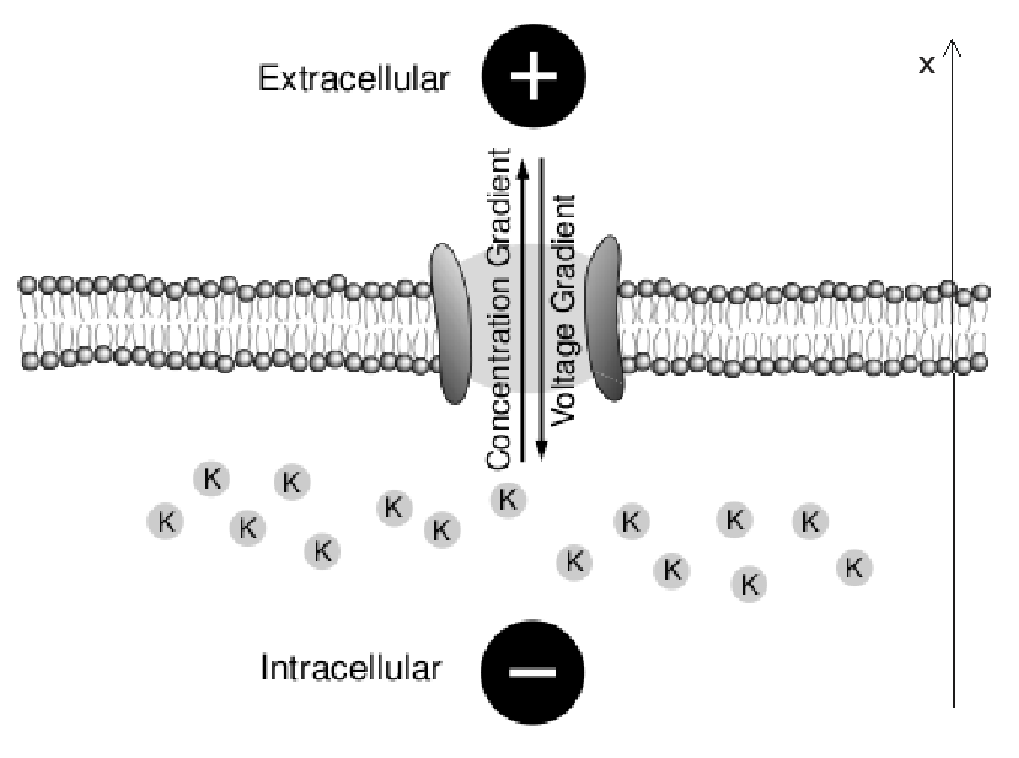
\includegraphics[height=6cm]{./images/membrane_battery.eps}}
  \caption{The basis of ionic battery}\label{fig:membrane-battery}
\end{figure}

Due to the potential difference between the two sides of the plasma
membrane, the ion channels can functions as an ionic battery, as shown
in Fig. \ref{fig:membrane-battery}. This creates an electric field
$\vec{E}$ which exert a force (called {\it drift} or
{\it electrophoresis}) on the charges near the channels. Although the
drift accelerate the ions moving across the membrane, it does not
accelerate forever. When the ions' velocities increase, the ions also
experience more collisions with each other. In the end, they attain an
average terminal velocity called a {\it drift velocity},
$v_{drift}$\footnote{\url{http://hyperphysics.phy-astr.gsu.edu/hbase/electric/ohmmic.html}}. This
drift velocity is on the order of millimeters per second ($\mu m/s$)
in contrast to the speeds of the electrons themselves which are on the
order of a million meters per second ($Mm/s$).  Assuming we're
examining the x-direction, if the electric field $\vec{E}$ is not so
strong, similar to eq.~\eqref{eq:137}, the drift velocity is
proportional to the field strength we have

\begin{equation}
  v_{drift} = \mu_p |\vec{E}|_x = -\mu_p \frac{\partial \Psi}{\partial x}
\end{equation}
with $d\Psi=\Psi_i-\Psi_o$, [$v_{drift}$]=[m/s], $\mu_p$
[m$^2$.(V.s)$^{-1}$] is the electrical mobility coefficient ($\mu_p
\lessgtr 0$) and $|\vec{E}|_x$ is the field strength ([V.m$^{-1}$]) in
the x-direction.  Then, the expression for the flux of ions due to
drift (or electrolyte) is

\begin{equation}\label{eq:J_elec}
  J_{drift} = J_{elec} = v_{drift} c = -\mu_p c \frac{\partial \Psi}{\partial x}
\end{equation}
with [$J_{elec}$] = [mol.s$^{-1}$.m$^{-2}$],$z$ is the valence of
charges [unitless], the concentration $c$ is [mol.m$^{-3}$].

Einstein, in 1905, showed that diffusion and drift experience the same
frictional resistance in
solution\footnote{\url{http://www.as.wm.edu/Faculty/DelNegro/cbm/050908.html}}.
Hence, the relation between the mobility and the diffusion is given by
\begin{equation}
  \label{eq:44}
  D = \mu_p \frac{k_BT}{q}
\end{equation}
with $q=ze$ is the charge carrier.  Eq.~(\ref{eq:44}) is the
{\bf Einstein equation} relating the electrical mobility $\mu_p$ to
the diffusion coefficient $D$. This equation is derived from ideal gas
equation, hence it is true for {\it ideal gas} only. However, Einstein
equation is a good approximation for electrolytes (particles are
ions).  In particular, mobility is not strictly constant and is
independent of the field strength $|\vec{E}|$.


% Hence, the expression for diffusion is
% \begin{equation}
%   \label{eq:63}
%   J_{diff} = J_{chem} = \mu_p \frac{k_BT}{q} \frac{\partial c}{\partial x}
% \end{equation}

The total flux
\begin{equation}
  \label{eq:89}
  J_{total} = J_{chem} + J_{elec} = -\mu_p \frac{k_BT}{ze}
  \frac{\partial c}{\partial x} - \mu_p c \frac{\partial \Psi}{\partial x}
\end{equation}
is the {\bf Nernst-Planck molar flux equation}.

Noting that $R = k_BN_A$ and $F=eN_A$ with $N_A$ is Avogadro number, we
have
\begin{equation}
  \label{eq:90}
  J_{total} =  -\mu_p \frac{RT}{zF}
  \frac{\partial c}{\partial x} - \mu_p  c \frac{\partial \Psi}{\partial x}
\end{equation}

If we multiply both side of eq.~(\ref{eq:90}) by $zF$ ($z$ is the
valence, $F$ is the Faraday's constant) which changes the flux of
material to flux of charge (which is by definition, electric current),
the result would be the current density.
\begin{equation}
  \label{eq:91}
  I = zFJ_{total} =  -\mu_p RT
  \frac{\partial c}{\partial x} - \mu_p Fz c \frac{\partial \Psi}{\partial x}
\end{equation}
with the current density [I] = [A/cm$^2$] =
[C.s$^{-1}$.cm$^{-2}$]. This is called
{\bf Nernst-Planck current density equation} and is more useful from
the perspective of neurophysiology.


\begin{figure}[htb]
  \centerline{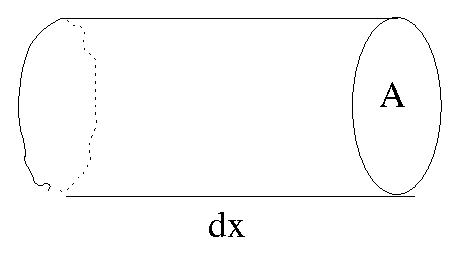
\includegraphics[height=3cm]{./images/cyllinder.eps}}
  \caption{Imaginary cylinder}\label{fig:cyllinder}
\end{figure}

\subsection{Derive Einstein equation}
\label{sec:derive-einst-equat}

We have introduced the Einstein equation in eq.~\eqref{eq:44}. Here,
we describe how to obtain this formula.

Now, we consider an imaginary cylinder of cross-section area $A$ and
length $dx$ containing an amount of charge particles. Assuming the
concentration of charge particles is $c$, then the number of particles
in the cylinder is $cAdx$.

Assuming each particle has an electrical charge $q$, then each will
exert a force $Eq$ on another ($E$ is the magnitude of the electric
field). Then the total electrical force is
\begin{equation}
  \mathcal{F}_{elec} = EqcAdx
\end{equation}

It's important to know that the increase in concentration
$\longleftrightarrow$ increase in pressure.  Then, with different
concentrations at two ends of the cylinder, we will have different
pressures (say $P+dP$ and $P$) at the two ends. This gradient in
concentration causes a chemical force
\begin{equation}
  \mathcal{F}_{chem} = A[(P+dP) - P] = AdP
\end{equation}

At equilibrium, the two forces will be of the same magnitude (but
opposite direction), then
\begin{equation}\label{eq:EqC}
  Eqc = \frac{dP}{dx}
\end{equation}

Remind from equation \eqref{eq:idealgas}, the ideal gas equation
\begin{equation}
  PV = Nk_BT
\end{equation}
with N is the number of charge particles. Since $\frac{N}{V}$ is
simply the concentration $c$.  Then
\begin{equation}
  P = ck_BT
\end{equation}
Apply it to \eqref{eq:EqC}, we have
\begin{equation}
  Eqc = k_BT\frac{dc}{dx} = k_BT\frac{\partial c}{\partial x}
\end{equation}

Furthermore, at equilibrium, the total flux is zero, then
\begin{equation}\label{eq:2flux}
  -D \frac{\partial c}{\partial x} = \mu_p c \frac{\partial
    \Psi}{\partial x}
\end{equation}

Since $k_B$ and $T$ are constants, and $E=-
\frac{\partial \Psi}{\partial x}$, combining eq.~(\ref{eq:EqC}) with
eq.\eqref{eq:2flux}, we have
\begin{equation}
  \mu_p = \frac{qD}{k_BT}
\end{equation}
or
\begin{equation}
  \label{eq:134}
  D = \frac{\mu_p k_BT}{q}
\end{equation}
In addition, by taking the antiderivative of eq.~(\ref{eq:2flux}), at
equilibrium, we have
\begin{equation}
  \label{eq:210}
    D \int_{in}^{out}\frac{dc}{c} = -\mu_p \int_{in}^{out}d\Psi
\end{equation}
or
\begin{equation}
  \label{eq:211}
  D \ln\frac{c_o}{c_i} = -\mu_p(\Psi_o-\Psi_i)
\end{equation}
or
\begin{equation}
  \label{eq:212}
  \frac{k_BT}{q} \ln\frac{c_o}{c_i} = (\Psi_i-\Psi_o) 
\end{equation}
or
\begin{equation}
  \label{eq:213}
  V_m = \Delta \Psi =   \frac{k_BT}{q} \ln\frac{c_o}{c_i} 
\end{equation}
with is the so-called {\bf Nernst equation}.

{\bf Example}: If there are two types of ions in the solution
(\ce{Na+},\ce{Cl-}).  Suppose that the initial concentration of the
two types of ions are equal and is denoted by $c$. Utilizing
eq. \eqref{eq:J_chem} and \eqref{eq:J_elec}, the net flux of ions
through the plasma membrane under the influence of ionic concentration
gradient and electric field is

\begin{equation}
  \label{eq:92}
    J_{total} = -(D_+-D_-) \frac{dc}{dx} - (\mu_++\mu_-) Ec
\end{equation}
with $E=\frac{\partial \Psi}{\partial x}$ is the scalar value of the
vector electric field $\vec{E}$.

{\bf NOTE}: The positive direction is assumed to be from inside to
outside (or from left to right). The plus (+) sign in the final
parentheses are due to the two species of ions, carries
opposite-signed but move in opposite direction, so contribute to the
current are additive.

Suppose there is only $n=1$ moles of charge particles, then
$q=nzF=zF$. Thus, we multiply two sides of eq.~(\ref{eq:92}) by the
charge $q$, we obtain the electric current (by our convention, in the
direction from inside to outside) is
\begin{equation}
  I = -q (D_+ - D_-) \left( \frac{\partial c}{\partial x}\right) - qEc(\mu_+ + \mu_-)
\end{equation}
which is called {\bf Nernst-Planck equation}, the same as
eq.~(\ref{eq:91}). This is the very important equation.  Then
\begin{equation}
  I =  -qc(\mu_+ + \mu_-)\left[ \frac{(D_+ - D_-)}{\mu_+ + \mu_-}
    \left( \frac{dc}{c}\right) + E \right]
\end{equation}
The second term inside the brace is the electric field. By analogy,
the first term should be the non-electric field (i.e. chemical field)
which arise naturally from the concentration gradient.  This is the more
general form of Ohm's law.
\begin{equation}
  I = -\sigma (E_{chem} + E)
\end{equation}
with $\sigma = qc(\mu_+ + \mu_-)$ and
\begin{equation}
  \label{eq:132}
  E_{chem} = q \frac{(D_+ - D_-)}{\mu_+ + \mu_-}
    \left( \frac{dc}{c}\right)
\end{equation}

\section{3. Membrane Domains}
\label{sec:membrane-domain}


``Self-replication systems require boundaries''

The cell membranes are not homogeneous in function, but localized in
regions of specialized functions.  The term `` domain or microdomain ``
is used to refer to such regions, marked distinctively from the
contiguous membrane by some physical features.

A lipid domain, which includes lipid caveolaeand lipid raft, are one of the
least understood membrane domains. They are rich in sphingolipids and
cholesterol  - thus also called cholesterol-sphingolipid-rich lipid domain.

\subsection{Lipid rafts}
\label{sec:lipid-rafts}


Lipid rafts can include/exclude proteins to variable extents. 
\begin{itemize}
\item	Glycosyl phosphatidylinositol (GPI - Sect.\ref{sec:GPI})-anchored protein,  
\item	Src-family kinases (double acylated proteins), 
\item	alpha-subunit of heterotrimeric G proteins 
\item	Cholesterol-linked and palmitoylated proteins (Hedgehog) 
  are the proteins with raft affinity.
\end{itemize}

Raft lipids are most abundant at the plasma membrane, but also found in the biosynthetic and endocytic pathways. 
\begin{itemize}
\item 	Cholesterol is synthesized in the ER.
\item	Sphingojlipid synthesis and head-grop modification occur in the Golgi.
\end{itemize}
It is suggested that first cholesterol-sphingolipid-raft first
assembled in the Golgi; and they move mainly towards the plasma
membrane.

\subsubsection{GPI-anchored protein}
\label{sec:gpi-anchored-protein}

GPI-anchored proteins are uniformly distributed on the cell
surface. However, under the expose to cross-linking antibodies, they
become clustered. 


\subsection{Lipid caveolae}
\label{sec:lipid-caveolae}

Lipid caveolae is a subset of lipid rafts found in the caveolae  - the
cell surface invaginations.

\section{4. Junctions between Plasmamembrane and ER-membrane}
\label{sec:junction-ER-plasmamembrane}
\label{sec:junction-plasmamembrane-ER}

The junction that connects the endoplasmic reticulum (Chap.\ref{chap:ER}) to the
plasma membrane (ER-PM junction) is unique in providing a direct communication
link between the ER and the PM.
The word {\it junction} whose etymologic origin is the Latin verb {\it jungere},
to join is used to define
\begin{itemize}
  
  \item  small gap: specialized parts of the ER and PM where the two membranes
  stay in close apposition and the width of the inter-membrane space ranges from
  7 to 30 nm

Electron micrograph (EM) images on T cell showed the gap as 17nm.  
The dyad (in the cardiac myocyte) or triad (in the skeletal muscle cell) is
about at a distance of 9 to 12 nm.

Under RyR-knockdown mice, the dyad junction is about 7nm.
Upon overexpression of JP-1 in nonmuscle cells, junctions of 7.6 nm are
observed, a distance similar to the 7 nm separating membranes in the junctions
of RyR knockdown mice


  \item no fusion: both membranes conserve their identity - fusion has not been
  observed.
  
  \item protein-rich region: it creates a restricted protein-rich cytoplasmic
  space.

  \item the membrane contact sites are stable from minutes to days
 
 Stable contacts differ from more transients contacts between the ER and PM that
 can
result from the continued highly dynamic remodeling of ER structures and those
that can bring membranes near each other without stable contacts necessarily
being formed.

\end{itemize}

Although ER-PM junctions were first described 50 years ago, their broad
importance in Ca2+ signaling, as well as in the regulation of cholesterol and
phosphatidylinositol lipid transfer, has only recently been realized.

The existence of contacts between the ER and the PM was first reported in 1957
in muscle and a few years later in neurons under EM images.
The best-characterized ER-PM junction is arguably the connection between the
sarcolemma (a muscle specialization of the PM) and the sarcoplasmic reticulum (a
muscle ER specialization) in cardiac and skeletal striated muscles.

Contacts between the ER membranes and the PM have received different names in the
literature
\begin{enumerate}
  \item dyad - Sect.\ref{sec:diadic_subspace} -- in cardiac myocyte
  
  \item triad - Sect.\ref{sec:triad} - in skeletal muscle cell
  
  \item PM-associated membranes, PM contact sites, peripheral
couplings, and ER-PM junctions
\end{enumerate}

\begin{mdframed}

Question: what is the signalling pathways or what is the structural connections
between the plasma membrane channels and the endoplasmic reticulum?
\begin{itemize}
  \item In myocyte: based on the concept in the skeletal muscle: DHPR channels
  on T-tubule interacts with RyR on SR membrane.

  \item In neurons:
   
In the phospholipase signaling system, endoplasmic reticulum IP3 receptors would
interact directly with plasma membrane capacitative calcium entry channels.

A fall in lumenal Ca2+ in the endoplasmic reticulum would induce a
conformational change of IP3R. This would be conveyed directly to the plasma
membrane channel via a protein-protein interaction that induces $\Ca$ entry,
which is called {\bf capacitative calcium entry}.

\end{itemize}

\end{mdframed}


The overexpression of the following proteins increase the number of
ER-PM junctions (as the ER calcium sensor)
\begin{enumerate}
  
  \item STIM (Sect.\ref{sec:STIM}): STIM1, STIM2

STIM associated with plasma membrane calcium channels Orai1-3
(Sect.\ref{sec:Orai}).

  \item junctophilin - Sect.\ref{sec:junctophilin}
  
  \item junctate - Sect.\ref{sec:junctate}
\end{enumerate}
However, the detail physiological components that required to form ER-PM
junction is not clearly known at different cell types.


{\bf NEURON}: Although neuronal ER-PM junctions were among the first to be
described in electron microscopy studies, their structure, components, or
functions are still not well understood.

{\bf YEAST, PLANTS}: Although yeast and plants have ER-PM junctions and Ca2+
signaling is essential for their physiology, none have STIM or Orai, and in the
case of yeast, the ER does not have a clear function in controlling Ca2+
homeostasis.

{\bf NON-EXCITABLE CELLS, e.g. lymphocyte}: 


\subsection{dyad}
\label{sec:dyad}

In cardiac cells, the junction between T-tubule (Sect.\ref{sec:t-tubule}) and
the junctional ER membrane is called a {\bf diads}, as the T-tubule and a {\it
single} terminal cisterna and it occurs at the Z-line.
% In cardiac cell, the SR coupling is {\bf dyads}, i.e. one SR terminal cisternae
% couple with T-tubule. 

This dyad is observed as a junctional area between the sarcolemma (T-tubular
surface) and flattened element of jSR (junctional SR) having 'feet' structure on
the surface \citep{carl1995}. 

The key components of a dyad is DHPR on one side
(Sect.\ref{sec:DHPR-Ca2+channel}) and RyR on the other side
(Sect.\ref{sec:ryr}). The cardiac-specific RyR isoform is RyR2.
Hower, the molecular component to form the dyad is more complex -
Sect.\ref{sec:junction-components}
\begin{itemize}
  \item dyad normal space is 9-12 nm
  
  \item dyad in RyR-knockdown mice: 7nm

It is not known if JP-2 only dyad can be stretched to 9-12nm; or it needs RyR.

\end{itemize}

A dyad is comprised of LTCC, RyR2, Cav3, and JPH2 in rat myocytes demonstrated a
temporal correlation between development of influx of Ca2+ from the LTCCa, CICR,
and T-tubule formation
\begin{itemize} 
  \item  JPH2 has also been shown to bind Cav3, a protein which localizes to the
sarcolemma

  \item Cav3 is necessary for the formation of 'little cave'-like invaginations
  of the cardiomyocyte sarcolemma called caveolae, as well as regulation of
  several cardiac ion channels including the LTCC and various K+ channels.
 
\end{itemize}

Whereas expression of Cav3 and RyR2 was observed early in development, JPH2
expression was not seen until day 15 and was associated with formation of the
T-tubule and maturation of CICR.

\subsection{triad: striated skeletal muscle}
\label{sec:triad}

The T-tubule (Sect.\ref{sec:t-tubule}), together with a {\it pair} of terminal
cisternae\footnote{the enlarged area of the SR} on either side and facing the
central T-tubule, form an arrangement known as {\bf triads}.
This is the location where local release of calcium occurs, i.e. $\Ca$ sparks
at the triadic junctions (Sect.\ref{sec:calcium-spark-skeletal-cell}).


Triadin, the protein found at the triad region, has been suggested maintaining
the linkage between DHPR and RyRs.
In skeletal muscle, the RyR isoform is RyR1 (Sect.\ref{sec:RyR}), which is
activated in triads by a voltage-triggered conformational change of DHPR that
induces the mechanical force to pull on the connected RyR1 to open the channel
and release Ca2+ from the ER into the cytosol - Sect.\ref{sec:VICR_CICR}.


\subsection{peripheral coupling: immature striated and
smooth muscles}
\label{sec:peripheral-coupling}

The functional couplings between the channels take place in junctional membrane
complexes (JMCs) called peripheral coupling in immature striated and smooth
muscles.

% Franzini-Armstrong, C. & Protasi, F. (1997) Physiol. Rev. 77, 699-729.
% 
% Flucher, B. E. (1992) Dev. Biol. 154, 245-260.

\subsection{smooth muscle ER-PM junction}

Guinea-pig urinary-bladder smooth muscle showed that RyRs and DHPRs can be
colocalized at ER-PM-like junctions. 
Though both calcium-dependent, contraction in smooth muscle is
slower in that of striated muscle (skeletal and cardiac) due to 
less numerous with a more random spatial pattern.

\subsection{yeast ER-PM junction}

The yeast ER structure differs from the one in mammalian cells.
Yeast ER can be separated into sheet-like perinuclear ER and cortical ER
structures, connected by ER tubules. The cortical ER is close to the plasma
membrane (PM) and forms numerous ER-PM junctions.

\subsection{rhabdomere (Drosophila) ER-PM junction}

Ommatidium: formed by eight photoreceptor cells that pack together to generate a
cone whose center is occupied by microvilli.

Rhabdomere ER-PM junction: an ommatidium showing photoreceptor cells (numbered;
only number 1 is shown fully in the Figure of Carrasco-Meyer (2011)) that extend
along the cone with the microvilli, constituting the rhabdomere.


\subsection{Components of a junction}
\label{sec:junction-components}s

Among the many proteins found in the ER-PM junctions
\begin{verbatim}
ER luminal protein: CSQ
RyR
Junctin
Mitsugumin29
Triadin
Junctophilin
JP45
Cytosolic protein: FKBP12.6 (associate RyRs)
DHPR
\end{verbatim}
DHPR, RyR, STIM1 are not required for forming ER-PM junction.

Junctophilin is the main candidate that play the important role of bridging the
membranes (Sect.\ref{sec:junctophilin}).

\textcolor{red}{\bf Translocation of ER-membrane proteins}:
ER-resident trans-membrane proteins typically have relatively high diffusion
coefficients that can range from 0.02 to 0.5 $\mum^2$/s (164, 165); 
with 0.05 $\mum^2$/s, STIM is among the slowest. This suggest for a period of 30
seconds, STIM1 range of action is finding junctions within approximately 2
$\mum$ radius.


\subsection{STIM (stromal-interacting molecule)}
\label{sec:STIM}

STIM is a ER-membrane protein that sense the change in ER calcium level and
involved in SOCE (Sect.\ref{sec:SOCE}).
There are two isoforms: STIM1 and STIM2. It is a calcium store sensor, i.e.
activated by $[\Ca]_\ER$-depletion and then interact with $\Ca$ channels on the
plasma membrane to trigger $\Ca$ influx.

There are two isoforms: STIM1 and STIM2.

\begin{enumerate}
  \item Calcium sensitivity: 
  
  STIM1 has high affinity to luminal calcium: $\approx 200 \muM$, i.e requires
  large reduction in ER calcium to be activated.
  
  STIM2 has a lower affinity to luminal calcium: $\approx 400 \muM$; i.e. thus
  STIM2 are partially activated at basal luminal calcium level.
  
  \item 
\end{enumerate}

Both STIM1 and STIM2 have consensus sequences for binding to EBs, and this
binding can be observed as a dynamic apparent movement of STIM1 with EB1 along
the ER membrane.

Both STIM isoforms also have a long coiled-coil
domain immediately adjacent to the membrane-spanning domain (split into two parts) that
may function as a spacer. It is estimated the length of this coiled-coil
domain is at least 15nm (based on the basis of about 0.14nm/amino acid spacing). 
This is about the gap of the spacing of the junction, i.e. about 17nm observed
in electron micrograph image of T cell.

\subsection{ -- STIM1}
\label{sec:STIM1}

STIM is a channel on ER membrane and is necessary for cells to trigger PM Ca2+
influx when ER Ca2+ levels decrease. At normal ER calcium level, STIM1 is kept
in an inactive state by the binding of Ca2+ in the ER to STIM1's EF hand in the
lumen of the ER. Inactive STIM1 is likely present in the ER in a monomeric or
dimeric form and Ca2+ dissociation from the EF-SAM domain triggers an increase in
oligomerization.


Upon low ER $\Ca$, it activates STIM1 and translocate STIM1 within the
endoplasmic reticulum to sites where it can interact with ion channels on PM.
At ER-PM junction, STIM1 interact with and open
\begin{enumerate}
  
  \item ORAI1 (Sect.\ref{sec:Orai}): activate the store-operated Orai1
  Ca2+-selective channels - (Sect.\ref{sec:SOC})
  

Orai1 can interact with STIM1 at the domain termed CAD  or SOAR domain, with the
domain likely forming a tetramer.
  
  
  \item STIM1 interacts with CaV1.2 channels when it is in the region of ER-PM
 junction having both CaV1.2 and Orai1 channels (Sect.\ref{sec:Orai})
 
 STIM1  activation can also be from mutational modification strongly suppresses
 voltage-operated calcium (CaV1.2) channels while activating store-operated Orai
 channels. 
  
\end{enumerate}


Translocation of STIM1 to ER-PM junctions likely occurs by passive local
diffusion over a few micrometers; via its interaction with PM PIP2 and
PIP(3,4,5)P3 lipids. \textcolor{red}{IMPORTANT}:
With 8 positive charges in monomeric STIM1, this is below the threshold of more
than 12 charges needed for cytosolic proteins to bind PIP2 and PIP(3,4,5)P3
lipids directly (Sect.\ref{sec:PIP2}). Thus oligomerization is considered
necessary; before translocation to occur.


{\bf IMPORTANT}: Oligomerization seems to be a key step in STIM1 activation.
However, it is not known how oligomerization of proteins occur as it can be
driven by either changes in ligand concentration or increases in the protein
concentration, possibly shifting the basal equilibrium state toward a partial
oligomerization in cells that overexpress STIM1.
\begin{enumerate}
  \item HYPOTHESIS OF $[\Ca]_\ER$-dependent STIM1 activation:

When Ca2+ in the ER is depleted, Ca2+ dissociates from the STIM1 EF-SAM domain,
changes its conformation, thereby inducing protein {\bf oligomerization},
generating a bigger cluster of positively charged amino acids; which is now
sufficient to interact with PIP2, and other negatively charged lipids in the PM.
This enables the localization of STIM1-PIP2 complex to the ER-PM junction; where
STIM1 can bind and activate Orai1 channel (Sect.\ref{sec:Orai}).

  \item [STIM1]concentration-dependent STIM1 activation:

Overespresion of STIM1 showed an increase in oligomerization; without needing
for reducing $[\Ca]_\ER$. Oligomerization likely leads to a loss in binding
between STIM1 and EB1 (end binding protein 1) proteins as suggested by an
observed loss in colocalization between STIM1 and EB1 following ER Ca2+
depletion.

\textcolor{red}{Oligomerization seems to be rapid, i.e. occur within 4seconds,
whereas STIM1 is still in the ER away from ER-PM junctions (from fluorescence
resonance energy transfer data)} (Carrasco - Meyer (2011)).
  
\end{enumerate}
% STIM1-localization change appears to be a reversible binding interaction
% with EB1 and not a processive STIM1-transport process

 
\textcolor{red}{Cell types}: STIM-Orai-mediated "inside-out" Ca2+ signaling is
found in in striated muscle excitation-contraction coupling, in directional
ergosterol lipid transfer from the ER to the PM in yeast, in
phosphatidylinositol (PtdIns) lipid transfer in Drosophila photoreceptor cells,
as well as in the creation of plasmodesmata cell-cell communication structures
in plants.

\begin{itemize}
  \item   {\bf YFP-tagged STIM1}: 
Lowering the level of Ca2+ in the ER induced the translocation of an
ER-localized YFP-tagged STIM1 protein to ER sites near the PM (puncta).
The translocation takes about 40 seconds, paralleling the induction of Ca2+
influx into cells.  No insertion of STIM1 to the PM was found.
YFP-STIM1 translocation to puncta could be rapidly reversed by again increasing
ER Ca2+. 
 
At the junction (Sect.\ref{sec:junction-ER-plasmamembrane}), STIM1 can stay in
the ER and signal to the PM by directly interacting with and 
\begin{enumerate}
  \item opening the PM-localized Ca2+ channel
  \begin{itemize}
 
     \item   Orai1 (Sect.\ref{sec:Orai}).
  
    \item  Trp channels  (Sect.\ref{sec:TRP-classification})
  
  This is not yet generally accepted. 
  \end{itemize}
  
  \item inhibiting CaLv1.2 (DHPR) - Sect.\ref{sec:DHPR-Ca2+channel}
  
  This is interesting in the context of muscle as discussed below, where STIM1
  may have a role in signaling a muscle 'fatigue state' when the sarcoplasmic
  reticulum (ER) level is too low and the muscle continue contraction. To
  increase interval of relaxation, i.e. contraction needs to be blocked;
  which is why the STIM-mediated inhibition of DHPRs may help with blocking
  the contraction and giving enough time for the reloading of the Ca2+ stores.
 
 
 \item regulate adenylate cyclase activity (Sect.\ref{sec:adenylyl-cyclase-classIII})
\end{enumerate}

When the concentration of Ca2+ inside the ER approaches an upper set point,
another protein, SARAF (TMEM66) associates with STIM1 to inactivate the
store-operated calcium channel

\end{itemize}

There are also hypothesis about the role of mitochondria as mitochondria can be
proximal to the PM and ER-PM junctions. Because the consequent Ca2+ increase in
the mitochondria is important for its metabolic activity, this may also suggest
that localized mitochondria near ER-PM junctions enhance a cell's ATP production
in response to Ca2+ influx.


\subsection{ -- STIM2}
\label{sec:STIM2}

Even though STIM2 is more likely to be activated than STIM1 (due to lower
affinity to calcium-binding inhibition effect), STIM2 is typically present at
much lower concentrations compared with STIM1.

STIM2 also has the lower maximal activation of Orai1 by STIM2 when compared with
STIM1.

The polybasic tail of STIM2 also has a higher affinity for PIP2 lipids compared
with STIM1, which may enhance its basal activity in cells. 





\subsection{junctophilin}
\label{sec:junctophilin}


Junctophilin is the protein believed to be important for bridging the ER-PM
membranes. (Review: Landstrom-Wehrens (2014), Carrasco-Meyer (2011)).

From the analysis of 60 JPH genes from over 40 species, Garbino et al. (2009)
confirmed the highly conservation of the gene across species.
% Molecular evolution of the junctophilin gene family
% Alejandro Garbino,1,2 Ralph J. van Oort,1 Sayali S. Dixit,1 Andrew P. Landstrom,3 Michael J. Ackerman,3 and Xander H. T. Wehrens1,2,4


\begin{enumerate}
  \item JP-1 found in skeletal muscle
  
  \item JP-2 : found in cardiac myocyte - Sect.\ref{sec:JP-2}

JP-2 knock-down mice showed JP-2 is required to constitute peripheral
coupling structures (the precursors of ER-PM junctions during myocyte
differentiation), though it is not sure the molecular-partner of JP-2 on the PM
is a protein or a lipid.
  
  \item JP-3 and JP-4: found in neuron
  (Sect.\ref{sec:JP-3})
\end{enumerate}

All have an ER transmembrane region and several MORN (membrane occupation and
recognition nexus) motifs in the sarcoplasmic-exposed region.
\textcolor{blue}{These motifs are necessary to link junctophilins with the PM}.
\begin{itemize}
  \item In plants:
  
These motifs can bind phosphatidic acid, phosphatidylinositol-4- phosphate, and
PIP2, thereby providing a possible mechanism for the connection between the ER
membranes and the PM.
 
  \item 
\end{itemize}

\subsection{-- JP-1}
\label{sec:JP-1}

JP-1 is expressed in skeletal muscle where ER-PM junctions are formed where
DHPR and RyR1 are also co-localized.


JPH1 plays a key role in skeletal muscle EC coupling and that disruption or
impairment of JPH1 function is associated with poor skeletal muscle function
through a loss of cellular ultrastructure and triad development.

Silcensing JP-1
\begin{enumerate}
  
  \item JP-1 knockout mice with perinatal lethality, mutant skeletal muscle
  shows deficiency of triad junctions and insufficient contraction.

  \item Disrupte the ER-PM junction, which is associated with impaired LTCC Ca2+ influx.

  \item Decreases store-operated Ca2+ entry (SOCE), which disturb the balances
  net Ca2+ loss from intracellular Ca2+ stores, leading to reduced
  SR-stored calcium release via RyR1.
  
  This is explained as the disruption of interaction between STIM1 and Orai1
  (Sect.\ref{sec:STIM1}).
  

  \item 
\end{enumerate}



\subsection{-- JP-2}
\label{sec:JP-2}

JP-2 is a member of the junctophilin family protein
(Sect.\ref{sec:junctophilin}) and is important for the formation of T-tubule-SR
junction \citep{21}. JP-2 expression can be silenced using JP-2 short hairpin
(sh) RNA. JP-2 shRNA can knock-out JP-2 expression level to 51\% after 64 hours
\citep{wei2010}.

JP-2 knockout embryos showing cardiac arrest, mutant cardiac myocytes exhibit
deficiency of peripheral couplings (Sect.\ref{sec:peripheral-coupling}) and
arrhythmic Ca2+ signaling. JPH2 null mice, although embryonic lethal,
demonstrate a 90\% increase in the distance of the cardiac dyad as well as
vacuolization of the SR. Mutations in JPH2, expressed in cardiocytes, cause
hypertrophic cardiomyopathy.

JPH2 expression silencing in cardiac cells in vitro has been shown to impair
CICR with decreased Ca2+ transient amplitude and blunting of spontaneous
generation of Ca2+ transients.
This was found in cells with unchanged expression of the LTCC, RyR2, NCX, SERCA,
and phospholamban and suggest JP2 silcensing altered function of RyR2 rather
than altered protein expression; 
\begin{enumerate}
  \item \sout{maybe through disrupting the junction
  which enables high elevation of subspace calcium to trigger RyR.}

WHY: Co-immunoprecipitation showed that RyR2 directly binds JPH2, suggesting a
role in the regulation of RyR2 gating.
  
  \item  (in JP2 knowckdown adult mice) increase RyR2 activity: RyR
  hyperactivity with increased spark frequency despite impaired CICR and EC
  coupling gain.

STUDY showed RyR2 clusters in close proximity to similarly shaped
clusters of JPH2 with approximately 80\% colocalization.
  
  \item 
\end{enumerate}


\subsection{-- JP-3 and JP-4}
\label{sec:JP-3}
\label{sec:JP-4}

Both JP-4 and JP-3 are found predominantly expressed in brain.

Unlike JP-1 and JP-2, JP-3 and JP-4 shows no signicant role in cellular
architecture stabilization and brain development individually. In particular,
JPH3 knockout mice had no discernible disruption in neuronal cellular
architecture.

Detailed intracellular Ca2+ signaling studies in these mice have not been done
to date, nor has a comprehensive analysis of all major functional regions of the
brain been done to determine whether a more robust phenotype may be
identifiable.

JP-3 is 
\begin{enumerate}
  \item  found to play a role in Huntington disease-like 2 (HDL2)
-Sect.\ref{sec:Huntington-disease}.
  
  \item JP-3 showed to play a role in mediating balance and motor control,
via maintenance of efficient calcium signaling.
 
  \item 
\end{enumerate}

JPH3/4 double knockout (JP-KDO) mice demonstrate disrupted intracellular Ca2+
signaling
\begin{itemize}
  
  \item   In Purkinje cells,  the JPH3 knockout mice demonstrated no apparent
  difference in action potentials and normal synaptic function.

JPH3/4 double knockout mice also demonstrate a similar impairment in Ca2+
signaling of Purkinje cells (as showed below).
It impaired Ca2+ crosstalk between plasmalemmal P/Q-type voltage-gated channels
and intracellular RyR channels impairing SK channel-mediated
after-hyperpolarization, i.e. low Ca2+ rise.

  \item disrupted communication between plasmalemmal Ca2+ entry via the
  N-methyl-D-aspartate (NMDA) glutamate receptors and intracellular neuronal
  RyRs, as well as the small conductance Ca2+-activated potassium (SK) channels,
  was noted in hippocampal neurons.

The molecular uncoupling of voltage-sensitive Ca2+ channels from neuronal RyRs
in JPH3/4-deficient mice may mirror the uncoupling of SOCE from RyR1 in skeletal
muscle with loss of JPH1.

\end{itemize}

[Kakizawa et al., 2008;
Garbino et al., 2009].

% \subsection{-- JP-4}
% \label{sec:JP-4}

JP-4 is found predominantly expressed in brain.
JPH4 localizes to spatially discrete areas in the brain compared with JPH3.


\subsection{junctate}
\label{sec:junctate}

Junctate is a Ca2+-sensing structural component of Orai1 and stromal interaction
molecule 1 (STIM1) - Sect.\ref{sec:Orai}, and Sect.\ref{sec:STIM1}.


\section{Biological property}
\label{sec:biol-funct-membr}

We have learnt the constituents of a plasma membrane
(Sect. \ref{sec:models-membranes}). In this and coming sections, we
will go into details its function.  Remembering that the constituents
of the biomembrane involve phospholipids, glycolipid, cholesterol,
integral proteins, peripheral proteins, as shown in
\ref{fig:membrane-full}.  The biomembrane is composed of 2 layers of
lipid molecules in which the hydrophobic ends of each layer face the
interior of the bilayer. This arrangement forms the semipermeability
in the lipids bilayer

\begin{figure}[htb]
  \centerline{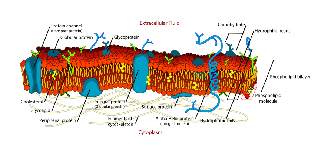
\includegraphics[height=6cm]{./images/Cell_membrane.eps}}
  \caption{Cell membrane composition}\label{fig:membrane-full}
\end{figure}

% bilayer of biomembrane
% At first, we will describe the biological functions of the cellular
% membrane. We also learnt that a thermodynamic system is stable only
% when the energy required to keep its components together is at the
% lowest possible value. And it requires much higher energy to keep a
% hydrophobic head stay closed to water molecules. Further, a lipid
% molecule is an amphipathic molecule with one hydrophobic group and one
% hydrophilic group.  In that sense, .

\subsection{Semipermeable}
\label{sec:semipermeable}


% special transmembrane proteins: active pumps & ion channels
As water can diffuse through the biomembrane, you might think that
small ions, e.g. \ce{Na+}, \ce{K+}, \ce{Ca^2+} can penetrate the
membrane easily. This is, however, incorrect since around the ions
there are always many surrounding water molecules and form the
{\it first solvation shell} (Sect.~\ref{sec:water}).  These water
molecules are electrostatically attracted to the ions because of the
relatively high surface-charged density of the ion. 

This make the ion moving as a shell with larger size than the ion's
size. So, in order to pass across the membrane, the ions need to break
all connections with the surrounding water molecules. This can be done
with the help of special transmembrane proteins which are classified
into two categories based on their selectivity: (1) {\it active pumps}
where more than one types of ions can pass through and it needs energy
(ATP), (2) {\it ion channels}, as shown in Fig.~\ref{fig:ion-channel},
where only a single type of ion can pass through and it does not
require energy, but is dependent on {\it electrochemical gradient}.
The former type is called {\it primary active transport}
(e.g. \ce{Na+}/\ce{K+}-ATPase, \ce{Ca^2+} ATPase), while the later
type is called
{\it secondary active
  transport}\footnote{http://en.wikipedia.org/wiki/Active\_transport}.
Each channel is indeed a specialized protein, of the generic family of
{\it major intrinsic protein} (MIP).

\begin{figure}[htb]
  \centerline{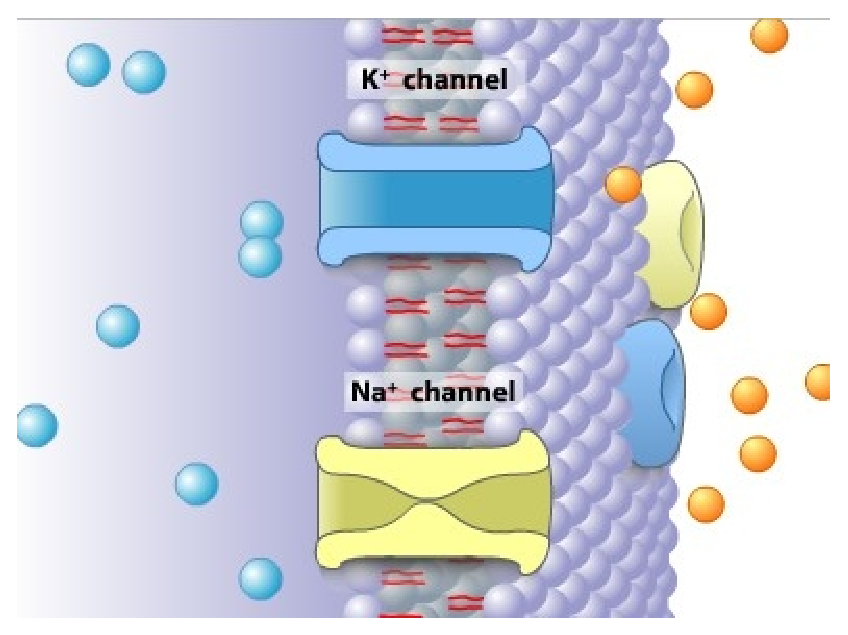
\includegraphics[height=6cm]{./images/ion-channels.eps}}
  \caption{Ion channels}\label{fig:ion-channel}
\end{figure}

The ions that we have mentioned
(\ce{Na+}, \ce{K+}) are particularly important for normal functions of
  the nervous signaling system. As these ions carry charges, their
  concentration define the {\it potential difference}  $V_m$
  between the cytoplasmic fluid and extracellular environment ($\Delta
  V = V_m = \Psi_i-\Psi_o$). We will study in detail the
  potential difference in section \ref{sec:electrical-property-biomembrane}.  

  \begin{framed}
    In
    myocytes, \ce{Ca^2+} is more important as it is considered as the
    second messenger agent, i.e. the change in its concentration in the
    cytoplasmic environment can trigger specific cellular
    events\footnote{\url{http://users.rcn.com/jkimball.ma.ultranet/BiologyPages/S/Second_messengers.html}}.
  \end{framed}
% %  and discuss in more detail in next
% % chapters that the change in potential difference between inside and
% % outside of biomembrane does ultimately stimulate a nerve spike.
% They may serve as second
% messenger agents, as the change in their concentration between
% extracellular environment and cytoplasmic environment can trigger
% specific cellular events.  

% \subsection{Primary active transports}
% \label{sec:prim-active-transp}

% Chap.~\ref{chap:nak-exchanger}. 

% \subsection{Ion-channels}
% \label{sec:ion-channels}



\section{Mechanical property}
\label{sec:mechanical-property-1}

The actual mechanical property of the plasma membrane is determined by
its physical properties, i.e. the composition. The composition is
different from membrane to membrane. Membranes with high proteins
content, e.g. of a mitochondrion (the protein-lipid ratio is 3:1),
tend to be stiff.  At region of lower protein content, like myelin
(the protein-lipid ratio is 1:10), it is highly flexibility.

You're recommended to read Chap.~\ref{chap:biom-prop-bio} first. 

\subsection{Foundation of mechanical physics}
\label{sec:found-mech-phys}

The tensile force $F$ is the stretching force pulling at both ends of
a component or structure along its length. The unit is [Newton], or
[N].
  \begin{figure}[htb]
    \centerline{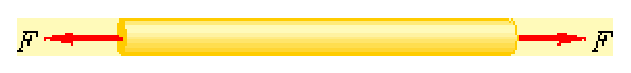
\includegraphics[height=0.5cm]{./images/tensileForce.eps}}
    \caption{Tensile Force F}\label{fig:tensileForce}
  \end{figure}

  This tensile force sets up a {\it tensile stress} (or
  {\it shear stress}) $\tau$ which is the applied force per a unit area of
  cross-section of a body. The unit is [Newton per unit area], or
  [N.m$^{-2}$].
  \begin{figure}[htb]
    \centerline{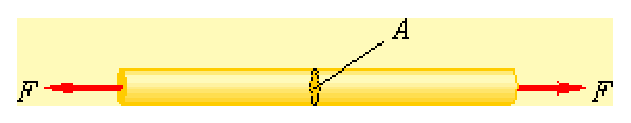
\includegraphics[height=1cm]{./images/tensileStress.eps}}
    \caption{Tensile Stress $\tau$}\label{fig:tensileStress}
  \end{figure}

\begin{equation}
  \label{eq:59}
  \text{tensile stress} = \tau = \frac{F}{A}
\end{equation}

The stress has the effect of stretching the object - a
{\it tensile strain} $\varepsilon$ (Cauchy strain, engineering strain) or the
increase of length per a unit of length. This quantity is unitless.
  \begin{figure}[htb]
    \centerline{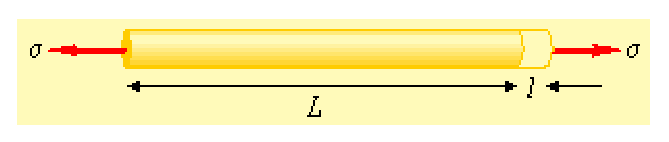
\includegraphics[height=1cm]{./images/strain.eps}}
    \caption{Strain}\label{fig:strain}
  \end{figure}

\begin{equation}
  \label{eq:58}
  \varepsilon = \frac{l}{L}
\end{equation}


Other properties of a structure:
\begin{itemize}
\item {\it elastic}: the ability of a structure to return to its
  original lengths after the load is removed. Such material can be
  distorted easily but does not break.

\item {\it strong}: a strong material needs high tensile force to
  break it, i.e. high breaking stress.

\item {\it stiff}:  a stiff material, in contrast to elastic one,
  needs a strong tensile force to produce a small extension (tensile
  strain), i.e. stiff material is difficult to change its shape. On
  the other hand, a {\it flexible material} only needs a small stress
  to produce a large extension.
\end{itemize}

The property of a material that tells us how stiff it is, within the
elastic limit, is called {\bf Young modulus}\footnote{\url{http://www.matter.org.uk/schools/Content/YoungModulus/Default.htm}}, denoted by Y.
\begin{equation}
  \label{eq:60}
  Y = \frac{\text{tensile stress}}{\text{tensile strain}} = \frac{\tau}{\varepsilon}
\end{equation}
the equivalent formula
\begin{equation}
  \label{eq:61}
  l = \frac{\tau}{Y}L
\end{equation}
is termed the {\it Hooke's law}.


{\bf Example}: extension vs. applied force on different materials in
Fig.~\ref{fig:extension-force}.
  \begin{figure}[htb]
    \centerline{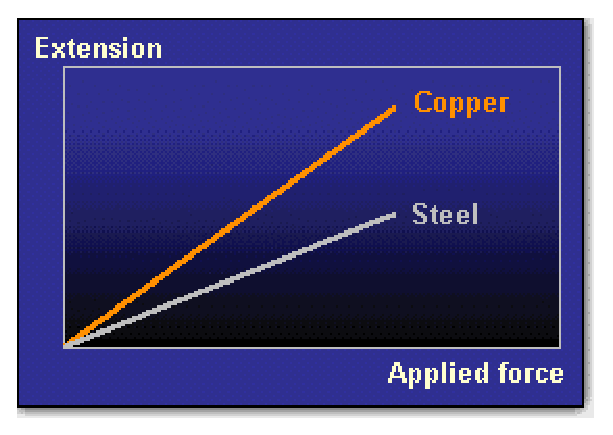
\includegraphics[height=4cm]{./images/extension-force.eps}}
    \caption{Extension-Force between copper and steel}\label{fig:extension-force}
  \end{figure}


\subsection{Mechanical property}
\label{sec:mechanical-property}


Mechanical properties of the biomembranes are very important for
understanding cell physiological functions (cell movements, cell
division, vesiculation, membrane fusion). These are controled by the
{\it visco-elastic properties of cell membranes}.

The lipids in the biomembranes show a high lateral mobility since they
can easily exchange their positions on one side of the plasma
membrane. The time interval for such lateral movement vary widely
(from minutes to many hours are known) depending upon the types of
lipids. The lipids can also exchange between the two leaflets of the
membrane. This is a so-called flip-flop process. The mobility of
transmembrane proteins, however, are strongly limited by their fixation
on the cytoskeleton.

It's important to know that physical parameters like viscosity,
elasticity, strain... are not suitable to represent highly organized
supramolecular structures like biomembranes.  Nevertheless, in some
cases, we still can use them as effective parameters (i.e. to have an
estimate of the system).

To examine the physical properties of the membrane, we consider a
tensile force F, as shown in Fig. \ref{fig:stress_motion}, to
extend/deform a membrane of surface area $A$ with length $l$ by an
amount $\Delta l$ which corresponds to a change in surface area
$\Delta A$.  In general, the biomembrane is easily {\it deformable} by
a shearing force causing a strain $\varepsilon$
\footnote{\url{http://en.wikipedia.org/wiki/Strain_(materials_science)}}.
\begin{equation}
  \label{eq:25}
  \varepsilon = \frac{\Delta l}{l}
\end{equation}

\begin{figure}[htb]
  \centerline{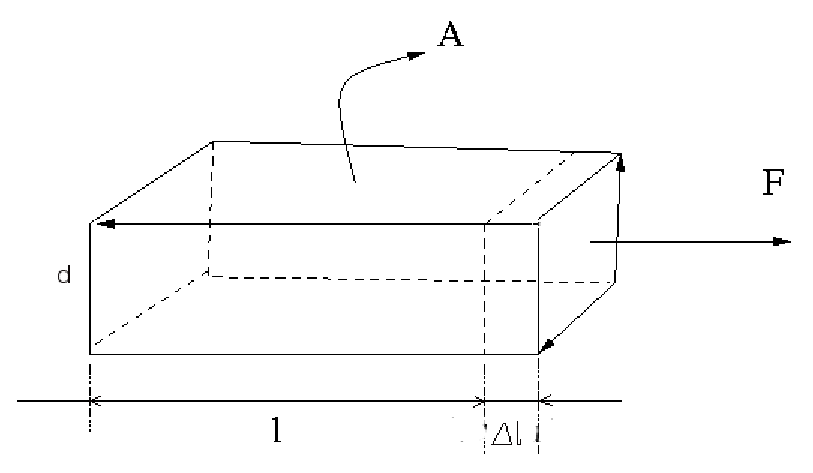
\includegraphics[height=6cm]{./images/stress_motion.eps}}
  \caption{Stress}\label{fig:stress_motion}
\end{figure}

To measure the stiffness, we use {\it Young's modulus}. Based on
eq.~\eqref{eq:60}, the stress $\tau$ is given as follows
\begin{equation}
  \tau = Y \frac{\Delta l} {l} = Y \frac{\Delta A}{A}
\end{equation}
% To establish a relationship between mechanical membrane properties and
% macroscopic materials (rubber, steel...), $Y'$ must be divided by the
% thickness of the membrane ($d$), which is approximately $d =
% 8\times10^{-9} m$, $Y = Y'/d$ [N.m$^{-2}$] which is called
% {\bf Young modulus}.
% The strain: $\varepsilon = \frac{\Delta l}{l}$ Hook's law tell us the
% stress: $\delta = Y.\varepsilon$.
\begin{table}
\begin{center}
\label{tab:sample-young-modulus}
  \begin{tabular}{|l|c|}
    \hline
    & Y \\
    \hline
    rubber & $10^6$ \\
    steel & $10^{11}$ \\
    membrane & $10^8$ \\
    \hline
  \end{tabular}
\caption{Sample Young modulus}
\end{center}
\end{table}

Looking at Table \ref{tab:sample-young-modulus}, surprisingly,
\textcolor{red}{the membrane is more bendable, flexible than
  rubber. However, membrane is not expandable}
($\varepsilon=0.02$). Specifically, the membrane will rupture if it is
expanded by more than 1-2\% of its area. This is due to the fact that
the bilayer is not chemically linked, but just a physical arrangement
under specific constraints. So, an increasing in area would lead to
the increase in distances between lipid heads which may hazardously
destroy the bilayer structure.

\begin{figure}[htb]
  \centerline{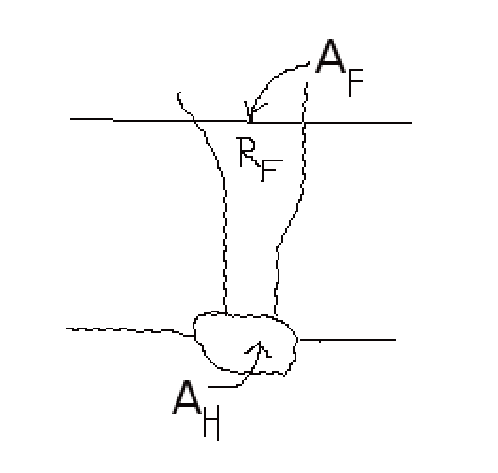
\includegraphics[height=5cm]{./images/single-lipid.eps}}
  \caption{Single lipid}\label{fig:single-lipid}
\end{figure}

If one leaflet of the membrane increases its area by an inclusion of
additional molecules. It's likely to form a conically-shape of lipid
molecules. A factor $f$ that characterizes this property relates the
area of the head groups ($A_H$ = constant) to the mean area ($A_F$),
as shown in Fig.\ref{fig:single-lipid}. In which $A_F$ can be
calculated by the mean length $l$ of the fatty-acids and the effective
volume of the region of fatty-acids ($V_F$) by: $A_F = V_F/l$. The
shape factor $f$ is defined as
\begin{equation}
  f = \frac{V_F}{lA_H}
\end{equation}
where $V_F$ strongly depends on their phase condition (i.e. degree of
order).

In summary, the membrane has very high flexibility in transformation
its shape, but with minimal ability for area extension. Indeed, it is
nearly impossible to extend the area of the membrane which is very
unlike rubber sheet.


\subsection{Surface tension $\gamma$}

As described in Fig. \ref{fig:air_water}(A), in bulk phase, each water
molecule can form up to 4 hydrogen bonds with other water
molecules. This interaction, between molecules of the same kind, is
referred to as {\bf cohesive
  force}\footnote{otherwise,
  it is called adhesive force}.
For a molecule in bulk, the cohesive force is shared equally to the
neighboring molecules, i.e. the molecule is pulled equally in all
directions.  Water molecules at the surface, however, can only form 2
hydrogen bonds on average. As a
result, % the force from the apical side is different from
% the other side. Hence, 
the water molecules at the water-air (or in
general, liquid-gas) surface experience stronger inward/downward
attraction forces and thus, tend to move downward, as shown in
Fig.\ref{fig:air_water}(B).

\begin{figure}[htb]
  \centerline{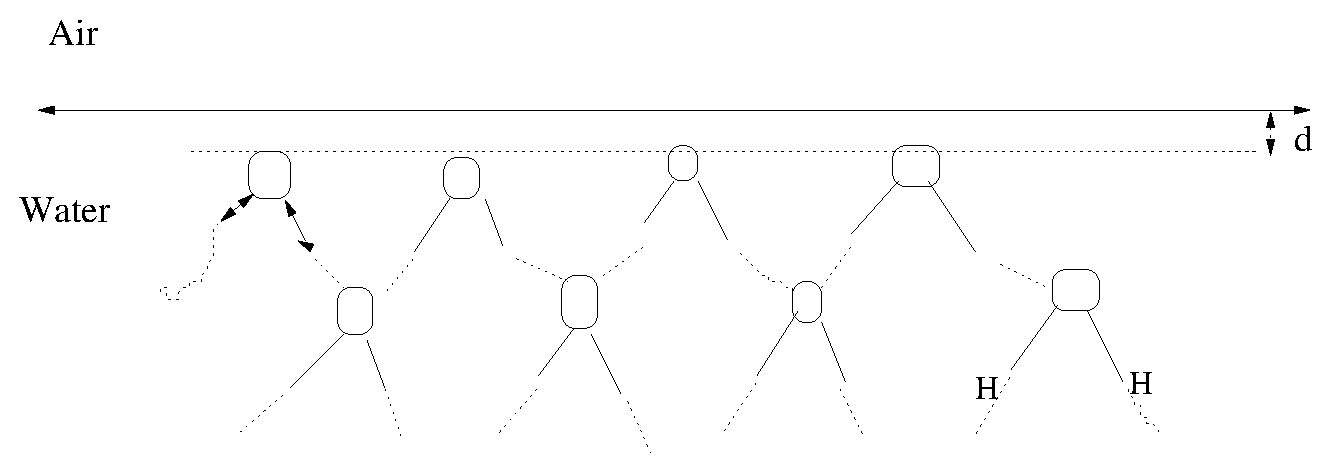
\includegraphics[height=3cm]{./images/air_water.eps},
    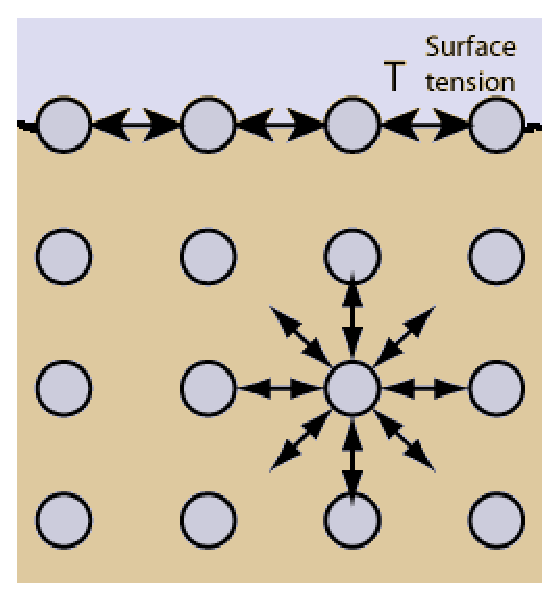
\includegraphics[height=3cm]{./images/cohesion-surface_tension.eps}}
\begin{center}
\verb|                 |(A) \verb|                            | (B)
\end{center}
  \caption{Water and Air intact}\label{fig:air_water}
\end{figure}



As described in eq. \eqref{eq:force-energy}, the higher the force in
interaction, the higher the magnitude of the energy. Hence, in order
to stay on the surface, the molecules on the surface must have a
higher energy than that of the molecules inside the bulk phase. We all
know that a system is stable only the energy is minimized. It means
that the aqueous system also tends to diminish the surface area
$S$. With minimal in surface area, this can reduce the number of water
molecules on the surface, or we can say it try to increase the number
of hydrogen bonds. 

However, this surface area cannot decrease to zero.  It means that the
cohesion forces between the molecules on the surface create a
repelling force against this inward attraction. This property is
referred to as {\bf surface tension}, denoted by $\gamma$. Its unit
can be 
\begin{itemize}
\item force per unit length, i.e. {\it dynes/cm}
\item {\it energy per unit area} (more general as it applies to not
  only liquid but also solid surface). This energy is called the
  {\bf surface energy}. The energy which is required to enlarge the
  surface of a liquid by 1$m^2$ is called
  {\bf specific surface energy} and is equivalent to the
  {\bf surface tension} $\gamma$ with [$\gamma$]=
  [J.m$^{-2}$]=[N.m$^{-1}$].
\end{itemize}

\begin{framed}
  If we want to increase the surface area, the system requires more
  and more liquid molecules at this higher level of energy (i.e. the
  surface energy).  It's important to know that
  {\it for objects with the same volume, the one with spherical shape
    has the minimum surface area}.
  This explains the behavior of bubbles or vesicles formation in
  liquids.
\end{framed}


{\bf Example:} At room temperatures (25$^0$C), we have
\begin{center}
  \begin{tabular}{|l|c|}
    \hline
    % \caption{Coefficient of tension}
    & $\gamma$ [N.m$^{-1}$] \\
    \hline\hline
    water & 0.0728 \\
    ethanol & 0.0223 \\
    benzene & 0.0282 \\
    \hline
  \end{tabular}
\end{center}
It's noting that the surface tension will decrease when the
temperature is increased.  Surface tension is important in two ways:
small organism can stand on the lakes surfaces; secondly, it's
important in biomechanics of the lung, where a highly solvated surface
is in contact with the air.

{\bf Example:} Now, we consider an example that the surface
surrounding a water environment is of spherical shape of radius
$R$. Due to surface tension, there will be an outer layer of width $d$
without any water molecules ($d\ll R$). We define:
\begin{itemize}
\item $V$ : volume of the sphere
\item $V_s$: volume of the outer layer (spherical shell)
%\item $V_s$: volume of the sphere ($=V + V_d$)
%\item $r$ : radius of the inner spherical container ($r \approx R$)
\end{itemize}
\begin{figure}[htb]
  \centerline{\includegraphics[height=3cm]{./images/sphere_water.eps}}
  \caption{Spherical aqueous environment}\label{fig:sphere_water}
\end{figure}
Then, the volume $V$ of the sphere and that $V_s$ of the spherical
shell, as shown in Fig. \ref{fig:sphere_water} are
\begin{equation}\begin{split}
    V = \frac{4}{3} \pi R^3 \\
    V_s \approx S.d = 4\pi R^2 d
  \end{split}
\end{equation}
given that $d \ll R$.

As the water molecule is small enough, we can assume that the water
molecules occupy all the spaces inside the spheres, then the ratio
\begin{equation}
  \frac{N_d}{N} = \frac{V_s}{V} \approx \frac{d}{R}
\end{equation}
with $N$ and $N_d$ are the number of water molecules to occupy the spherical
container and spherical shell, respectively.

% For any sphere, at the outer layer, the value of $d$ is quite constant
% (fixed). So, when $R\rightarrow \infty$, we will have $N_d \ll N$.
% So, if we examine a very small sphere with a few water molecules. The
% radius R has the tendency to increase.

\begin{figure}[htb]
  \centerline{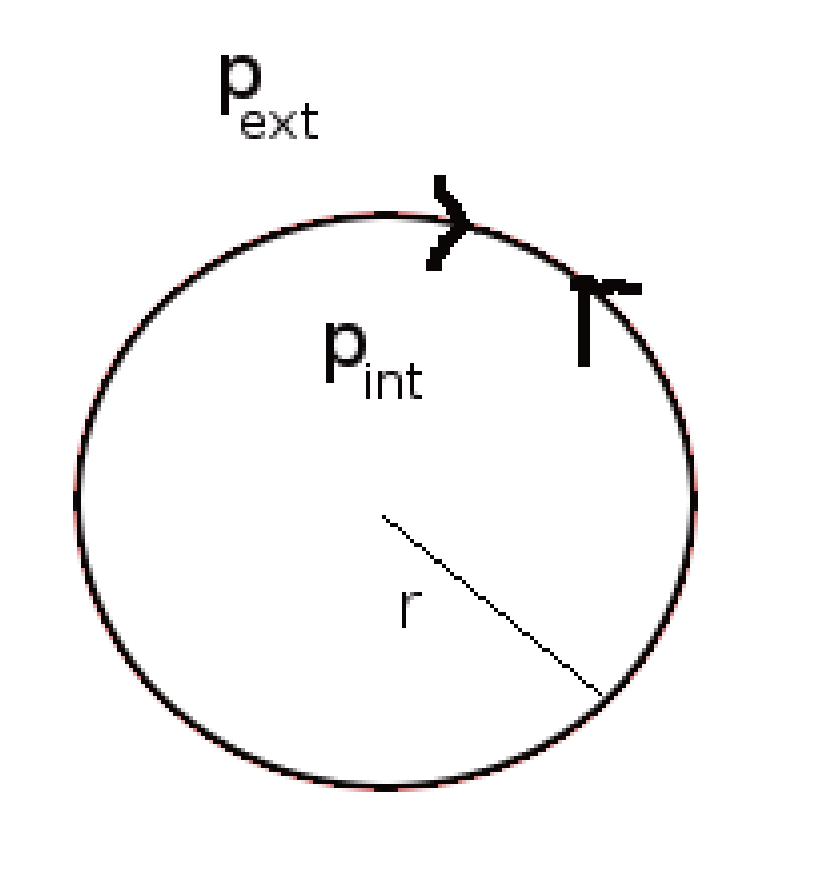
\includegraphics[height=3cm]{./images/buble.eps}}
  \caption{A vesicle with a surface tension $\gamma$}\label{fig:buble}
\end{figure}


Now, we consider an air bubble (vesicle) inside the water
environment. The water tension causes a pressure $p_{ext}$ on the
surface of the vesicle and decreases the volume of the vesicle and
in turns generates a repelling pressure $p_{int}$, as shown in
Fig.\ref{fig:buble}.  Given the unit of the surface tension $\gamma$
is energy per unit of area [J.m$^{-2}$], under the exerting force
$f_s$, the vesicle possesses a potential energy $E_s$ 
\begin{equation}
  E_s = \gamma \text{S} =  \gamma 4\pi r^2
\end{equation}
with S is the surface area, and $\gamma$ is also called the
coefficient of the surface tension of the vesicle.  Then, the exerting
force, in the opposite direction of $E_s$, is
given as\footnote{\url{http://hyperphysics.phy-astr.gsu.edu/HBASE/pegrav.html}}

\begin{equation}
  f_s = - \frac{\partial E_s}{\partial r} = - 8 \pi r \gamma
\end{equation}
and accordingly, the pressure (the force per unit area) on the vesicle
is
\begin{equation}
  p_s = \frac{f_s}{\text{S}} = - \frac{ 8 \pi r \gamma}{4\pi r^2} = - \frac{2\gamma}{r}
\end{equation}
This is the difference between external pressure and internal
pressure, or
\begin{equation}
  p_s = p_{ext} - p_{int}
\end{equation}
Finally, we have
\begin{equation}
  p_{int} =  p_{ext} + \frac{2\gamma}{r}
\end{equation}
It is evident that, for a larger vesicle, the tension is reduced.



\section{Electrical Property}

Check Sect.\ref{sec:electrical-property-biomembrane}.

\section{Signaling pathways}
\label{sec:signaling-pathways}


Lipid metabolites are key elements in signaling pathways

Signal Transduction Knowledge Environment (STKE) is a comprehensive
resource for database on signaling pathways.

\subsection{Signal transmission}
\label{sec:signal-transmission}

{\bf Signal transduction} (previously, signal transmission or sensory
transduction) refers to the process of a cell convert one kind of
signal/stimulus to another.

Most signal transduction process involves a series of chemical
reactions.  Most signal transduction 



\section{MIP: Aquaporins}
\label{sec:aquaporins}
\label{sec:MIP-major-intrinsic-protein}

Aquaporins are water-specific transmembrane (TM) proteins and belongs to the
so-called {\bf major intrinsic proteins} (MIP). MIP family proteins are thought
to contain 6 TM domains. Genetic defects in Aquaporins have linked to several
human diseases. Peter Agre who discovered aquaporins was awarded Nobel prize in
2003, along with Roderick MacKinnon for his work on the structure and mechanism
of potassium channels. 

Water molecules can go inside the cells via aquaporins, with a much faster rate
than via the phospholipid bilayer. Transport via phospholipid bilayer is called
osmosis. In 1993, the first aquaporin (aquaporin-1 or previously called CHIP-28
as it has 28 kDa) was reported by Agre from John Hopkins University
\citep{agre1993}. Before that, no one has questioned of a second pathway for
water transport other than phospholipid bilayer due to the relatively high water
permeability in some epithelial cells.


% \chapter{Membrane Physics}
% \label{chap:membrane-physics}
% 
% In Chapter \ref{chap:membranes}, we have studied some very important
% properties of a biomembrane.


\section{Focal adhesion (cell matrix)}
\label{sec:focal-adhesion}

The focal adhesions (also cell-matrix adhesions or FAs) are large macromolecular
assemblies through which mechanical force and regulatory signals are transmitted
between the extracellular matrix (ECM) and an interacting cell.

The assembly of focal adhesions is highly regulated, with protein recruitment
occurring in a sequential manner, resulting in a structure with organized
layers.

\section{HEK293 cells}
\label{sec:HEK293-cell}

%%% Local Variables: 
%%% mode: latex
%%% TeX-master: "mainfile"
%%% End: 